%=========================================================================%
%   "Epigenetic basis of endocycle regulation in Oikopleura dioica"
%
% Master thesis by André Figueiredo Rendeiro
% 2013/1014
%
% University of Aveiro thesis
% based on the template by Tomás Oliveira e Silva
%
%=========================================================================%

\documentclass[11pt,twoside,a4paper]{report}
%incluir 'final' nas opções em baixo para omitir "Documento Provisório"
\usepackage[DBIO,newLogo,final]{uaThesis}

% packages
\usepackage[english]{babel}
\usepackage{hyperref}
\usepackage{amsmath}
\usepackage{amssymb}
\usepackage{xspace}% used by \sigla
\usepackage{cite}
\usepackage[titletoc]{appendix}
\usepackage{emptypage} % to remove numbering from empty pages
\usepackage{multirow} % for merging cells in tables
\usepackage{float} %to manage floating objects
\usepackage{array} % used in table
\usepackage{titlesec} % used to format paragraph sections
\usepackage{fancyhdr} % used to format headings and footer

\usepackage{caption}
\usepackage{subcaption}

\usepackage[section]{placeins}  % force figure position in section

% provide encoding packages depending on the compiler
\ifxetex
  \usepackage{fontspec}
\else
  \usepackage[T1]{fontenc}
  \usepackage[utf8]{inputenc}
  \usepackage{lmodern}
\fi
% to get external fonts (e.g. google webfonts)
% must use xelatex compiler!!!
% \setmainfont[Ligatures=TeX]{Junge.ttf}

% defs
\def\ThesisYear{2014}
\def\ThesisAuthor{André Figueiredo Rendeiro}
\def\ptThesisTitle{Bases epigenéticas da regulação de endociclos em Oikopleura dioica}
\def\enThesisTitle{Epigenetic basis of endocycle regulation in Oikopleura dioica}

% optional (comment to use default)s
%   depth of the table of contents
%     1 ... chapther and sections
%     2 ... chapters, sections, and subsections
%     3 ... chapters, sections, subsections, and subsubsections
\setcounter{tocdepth}{5}
\setcounter{secnumdepth}{5}

% make paragraphs look like sections
\titleformat{\paragraph}[hang]{\normalfont\small\bfseries}{\theparagraph}{1em}{}
\titlespacing*{\paragraph}{0pt}{3.5ex plus 1ex minus .2ex}{1em}

% heading and footer
\pagestyle{fancy}
\renewcommand{\headrulewidth}{0pt}
\fancyhf{}
\fancyhead[lo]{\slshape\nouppercase{\rightmark}}
\fancyhead[re]{\slshape\nouppercase{\leftmark}}

\lfoot[\thepage]{}
\cfoot{}
\rfoot[]{\thepage}

% custom macros (could also be defined using \newcommand)
\def\I{\mathtt{i}}         % one possible way to represent $\sqrt{-1}$
\def\Exp#1{e^{2\pi\I #1}}  % argument inside braces, i.e., "{}"
\def\EXP#1.{e^{2\pi\I #1}} % argument finishes when a full stop is encountered, i.e., "."
\def\sigla{\LaTeX\xspace}  % use as "blabla \sigla blabla (no need to do "blabla \sigla\ blabla"

\def\AddVMargin#1{\setbox0=\hbox{#1}%
                  \dimen0=\ht0\advance\dimen0 by 2pt\ht0=\dimen0%
                  \dimen0=\dp0\advance\dimen0 by 2pt\dp0=\dimen0%
                  \box0}   % add extra vertical space above and below the argument (#1)
\def\Header#1#2{\setbox1=\hbox{#1}\setbox2=\hbox{#2}%
           \ifdim\wd1>\wd2\dimen0=\wd1\else\dimen0=\wd2\fi%
           \AddVMargin{\parbox{\dimen0}{\centering #1\\#2}}} % put #1 on top #2

\newcommand{\degree}{\ensuremath{^\circ}}
\DeclareUnicodeCharacter{B0}{\degree}

\begin{document}

%=========================================================================%
% Cover page (use only one of the first two \TitlePage)
%=========================================================================%
\TitlePage
    \HEADER{%\BAR\
    }{\ThesisYear}
    
    \TITLE{\ThesisAuthor}
        {\ptThesisTitle}
    \vspace*{10mm}
    \TITLE{}{\enThesisTitle}
          %\HEADER{\BAR\FIG{\begin{minipage}{50mm} % no more than 120mm
          %``I'm King of the world.''
          % \begin{flushright}
          %  --- Jack Nicholson
          % \end{flushright}
          % \end{minipage}}}
          % {\ThesisYear}
\EndTitlePage

\cleardoublepage

%=========================================================================%
% Cover page
%=========================================================================%

\TitlePage
    \HEADER{}{\ThesisYear}
    \TITLE{\ThesisAuthor}
        {\ptThesisTitle}
    \vspace*{10mm}
    \TITLE{}{\enThesisTitle}
    \vspace*{15mm}
    
    \TEXT{}
       {Dissertação apresentada à Universidade de Aveiro para cumprimento dos requisitos necessários à obtenção do grau de Mestre em Biologia Molecular e Celular, realizada sob a orientação científica de Eric Thompson, Professor do Departamento de Biologia da Universidade de Bergen e de Manuel Santos, Professor Associado do Departamento de Biologia da Universidade de Aveiro.}
       
\EndTitlePage

\cleardoublepage

%=========================================================================%
% Title page
%=========================================================================%

\TitlePage
  \vspace*{55mm}
  \TEXT{\textbf{jury}}{}
       
  \TEXT{president}
       {\textbf{António MASADASDDSASD}\newline {\small Associated Professor at the Biology Department of the University of Aveiro }}
  \vspace*{5mm}
  
    \TEXT{}
       {\textbf{António MASADASDDSASD}\newline {\small Associated Professor at the Biology Department of the University of Aveiro }}
  \vspace*{5mm}
  
    \TEXT{}
       {\textbf{António MASADASDDSASD}\newline {\small
        Associated Professor at the Biology Department of the University of Aveiro }}
  \vspace*{5mm}
  
\EndTitlePage

\cleardoublepage

%=========================================================================%
% Dedications
%=========================================================================%

\TitlePage
  \vspace*{55mm}
    \TEXT{\textbf{acknowledgements}}
        {I thank Prof. Thompson for allowing me to work in his lab and for all help with my stay in Norway. Pavla, for unconditional support and guidance during this period, Gemma for irreplaceable computational help, and everyone in the lab for all the good laughs and help when needed.}
    \TEXT{}
        {I'd like to thank my family for all the support throughout these years, allowing me to follow my dreams.}
    \TEXT{}
		{I'd also like to acknowledge the free open source software community for its marvellous efforts in building an open world and Tomás Oliveira e Silva for the University of Aveiro \LaTeX thesis template.}
    \TEXT{}
        {This thesis was made using entirely free open source software.}


\EndTitlePage

\cleardoublepage

%=========================================================================%
% Portuguese abstract page
%=========================================================================%

\TitlePage
  \vspace*{55mm}
  \TEXT{\textbf{palavras-chave}}
        {epigenética, endociclos, Oikopleura dioica}
  \TEXT{\textbf{resumo}}
    	{Lorem ipsum dolor sit amet, consectetur adipisicing elit, sed do eiusmod tempor incididunt ut labore et dolore magna aliqua. Ut enim ad minim veniam, quis nostrud exercitation ullamco laboris nisi ut aliquip ex ea commodo consequat. Duis aute irure dolor in reprehenderit in voluptate velit esse cillum dolore eu fugiat nulla pariatur. Excepteur sint occaecat cupidatat non proident, sunt in culpa qui officia deserunt mollit anim id est laborum.}
\EndTitlePage

\cleardoublepage

%=========================================================================%
% English abstract page
%=========================================================================%

\TitlePage
    \vspace*{55mm}
    \TEXT{\textbf{keywords}}
        {epigenetics, endocycles, Oikopleura dioica}
  \TEXT{\textbf{abstract}}
		{Lorem ipsum dolor sit amet, consectetur adipisicing elit, sed do eiusmod tempor incididunt ut labore et dolore magna aliqua. Ut enim ad minim veniam, quis nostrud exercitation ullamco laboris nisi ut aliquip ex ea commodo consequat. Duis aute irure dolor in reprehenderit in voluptate velit esse cillum dolore eu fugiat nulla pariatur. Excepteur sint occaecat cupidatat non proident, sunt in culpa qui officia deserunt mollit anim id est laborum.}
\EndTitlePage

\cleardoublepage

%=========================================================================%
% Tables of contents, of figures, ...
%=========================================================================%

\pagenumbering{roman}

\tableofcontents

\listoffigures

\listoftables

\cleardoublepage
%=========================================================================%
% The chapters (usually written using the isolatin font encoding ...)
%=========================================================================%
\pagenumbering{arabic}
%=========================================================================%
\chapter{Introduction}
%=========================================================================%

	\section{Endoreplication, a polyploid cell cycle}
		Polyploid cells possess more than two pairs of their set of chromossomes. This polyploid state is common to be predominant within fungi, plants and some vertebrates like fish and amphibians, but also within restricted cell types in many other organisms \cite{Fox2013}.
		
		Documented advantages of polyploid organisms compared to diploids include heterosis (a evolutionary situation where the progeny has fitness advantages compared to its progenitors), gene redundancy, and gain of asexual reproduction by loss of self-incompatibility \cite{Comai2005}. From a strict cellular perspective, gene redundancy is the most relevant - it provides a way of masking the effect of deleterious alleles, and shields the possible effect of mutagens in the DNA. On the other hand, the increase of the gene-space available for mutations to act can also be seen as a evolutionary advantage.
		
		Changing ploidy within a cell has tremendous consequences for its physiology. Increased genetic material when active will produce more products, which will contribute to increase the cell volume and this inevitably changes the general cellular architecture. Higher number of genomic loci will bring new challenges in nuclear organization which can alter the epigenetic stability and consequently, gene expression. Cell division can be seriously compromised due to the inadequacy of the cell division machinery in dealing with an abnormal number of chromosomes. Like anything exposed to selection, only the sum of all these attributes will predict the outcome of the success of the organism, and while some of these events may be seriously restrictive to an organism survival in a specific environment, in others it might confer advantages.
		
		Polyploidy as a cellular state is known for more than a century, but studies of it under the light of endoreplication, a cell cycle mode which relies on cycles of genome replication without cell division (see Figure \ref{fig:simple_cell_cycle}), only recently began to gain relevance. Two main ways exist for the occurrence of endoreplication: endocycling, where genome replication in the S phase of the cell cycle alternates with a G phase preparing for the next replication; endomitosis, where an abortive mitotic cell division attempt after genome replication returns to a new G phase. Since the outcome of both is the same - the creation of a single polyploid cell - the distinction between the two can sometimes be unclear.
		
		\begin{figure}[here]
			\centering
			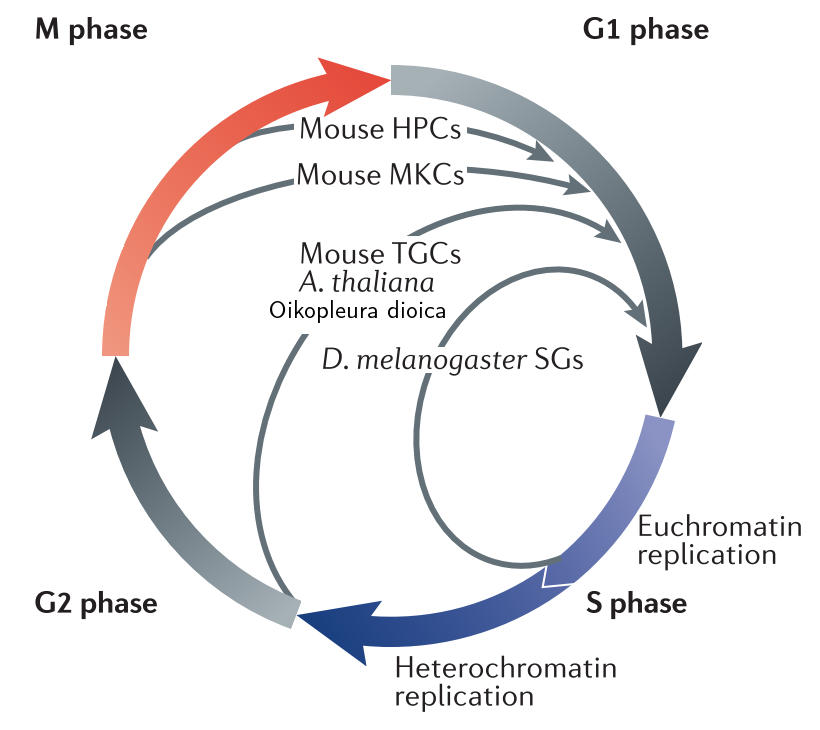
\includegraphics[width=0.6 \textwidth]{pngs/simple_cell_cycle.png}
			\caption{The eukaryotic canonical endoreduplicative cell cycles. {\footnotesize Adapted from \cite{Frisch2002}}}
			\label{fig:simple_cell_cycle}
		\end{figure}
		
		Most remarkably, the core protein machinery that drives and regulates the canonical mitotic cell cycle performs as well in endocycles.
		%Key signalling factors during development seems to exploit conserved cell cycle pathways to guide a cell into performing endocycling. 
		
			\subsection{An overview of the eukaryotic canonical cell cycle}
			Cell division is a mechanism common to all organisms, being necessary for reproduction and also used for growth and proliferation in multicellular organisms. Regulation of the whole cell cycle and cell division is intricately complex, but is necessary to assure progression into the several phases in a controlled manner. Multicellular eukaryotes in particular, require precise timing and sensing of internal and environmental clues, which is regulated by complex cellular machinery, to achieve correct tissue and organ development.
			
			The canonical cell cycle consists of four major phases: gap phase one (G1) - cell growth and synthesis of required subtracts for DNA synthesis; Synthesis (S) - genome replication; gap phase two (G2) - continued cell growth; mitotic phase (M) - cell division through mitosis. Progression through the cell cycle phases is controlled by a number of checkpoints where genomic and cellular integrity are attested and various internal and external cues are considered, allowing progression, or arresting cell cycle.
			
			Numerous protein classes interact during regulation of the canonical cell cycle, being the complexes formed by Cyclins and Cyclin-dependent kinases (CDK) very prominent. Different CDK-Cyclin complexes are activated throughout the cell cycle, and their specific temporal regulation allows modulation of the activity of specific downstream effectors of cycle progression. While CDKs remain relatively constant through the cycle, the level of the Cyclin subunit is regulated thus restricting the complexes' temporal activity. 
			
				\subsubsection{Cell cycle progression regulated by CDK-Cyclin complexes}
				In general, the overall activity of CDK-Cyclin complexes increases from G1 to M, being several thresholds of their activity used by the cell to identify the phase it is in.
								
				% some CDKs are mitotic, some are...
				The G1 phase is the one with lowest CDK-Cyclin activity. This allows the cell to start replication with the assembly of the replication-specific proteins into a pre-replication complex in DNA sites that will become origins of replication. The assembly of pre-replication complexes during the G1 phase licenses replication and when CDK activity is detected above a threshold, the S phase begins with DNA replication. High CDK activity activates replication but also prevents replication licensing during other phases, for it requires low activity. A unique cell division per cycle is thus assured, for only when CDK activity is abolished at the end of mitosis can the genome be licensed for replication again.
								
				In the G1 phase, the D cyclins are expressed in response to external cues such as growth factors. These associate with both CDK 4 and 6 and phosphorilate downstream targets which most importantly include the retinoblastoma protein (pRb). pRb natively binds to a complex formed by a member of the E2F family of transcriptions factors (TF) and DP (also a TF), inhibiting it. When phosphorilated, pRb releases the E2F-DP TF complex and this is free to bind DNA and activate the expression of downstream genes that are responsible for entry into the S phase (Figure \ref{fig:pRb-E2F}).
				
				\begin{figure}[here]
					\centering
					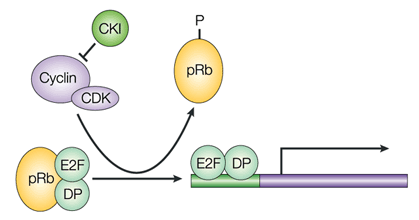
\includegraphics[width=0.5\textwidth]{pngs/CDK-pRb-E2F-DP.png}
					\caption{Cyclin-CDK phosphorilation of pRb and release of the E2F TF during G1 phase of the cell cycle. {\footnotesize Adapted from \cite{Frisch2002}}}
					\label{fig:pRb-E2F}
				\end{figure}
				
				Among the genes regulated by the E2F TF upon S phase entry is Cyclin A. This Cyclin first interacts with CDK2 and this complex is required for successful completion of S phase. Later, Cyclin A complexes with CDK1 having a function in G2/M phases transition.
				
				In the mitotic phase the predominant Cyclin-CDK complex is the Cyclin B-CDK1, which has important functions in phosphorilating cytoskeletal proteins involved in mitosis.
				
				Towards the end of cell division, cyclins are degraded, therefore greatly reducing the overall level of CDK activity. Both A and B cyclins are ubiquitinated by the ubiquitin ligase anaphase-promoting complex/cyclosome (APC/C), which includes the Fzr/Cdh1 subunit. This subunit confers Cyclin A and B specificity, marking them for proteolytic degradation starting at the end of mitosis but continuing through the G1 phase, which helps to ensure unidirectional cell cycle progression.	
				
				Cyclin-CDK activity can also be modulated by Cyclin-dependent kinase inhibitors (CKI). Among the most prominent are p27 which inhibits CDK4 in the pre-S phase Cyclin D-CDK4 complexes - therefore preventing phosphorilation of pRb and E2F release - and CDK 2 in the Cyclin E-CDK2 complex causing the cell to stay in S phase.
				
				Downstream effects of Cyclin-CDK activity involve activation of various cell cycle effectors including cyclins necessary for the subsequent phase, and this is fundamental for all cell cycle events to occur, specially in the beginning of the S phase, and during mitosis, assuring that the latter cannot start without the first and vice-versa, and that once they have started they cannot be reversed. These concepts can be visualized in Figure \ref{fig:canonical_cycle} and will prove useful when considering the implications of an endoreplicative cell cycle - a cycle of G and S phases.
				
				\begin{figure}[here]
					\centering
					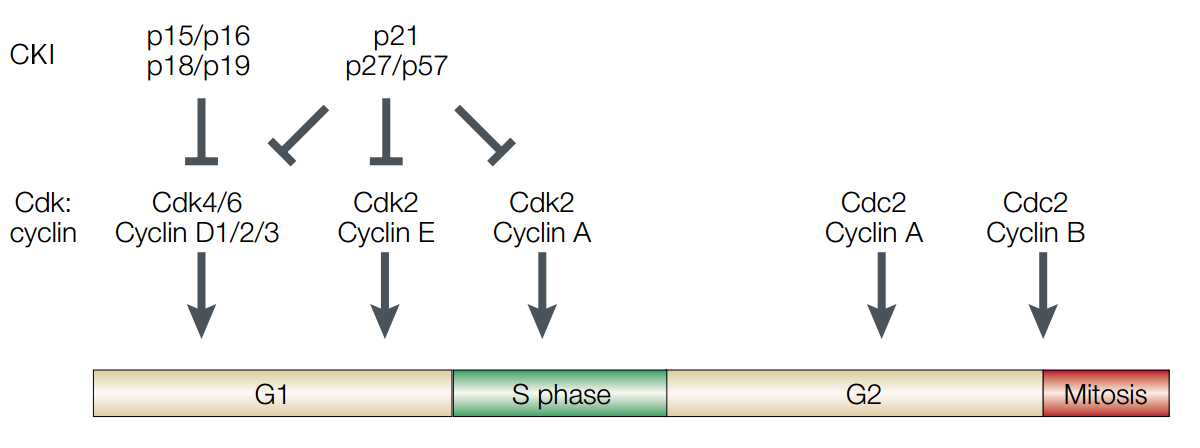
\includegraphics[width=0.9\textwidth]{pngs/canonical_cell_cycle.png}
					\caption{The phases of the canonical eukaryotic cell cycle. {\footnotesize Adapted from \cite{Trimarchi2002}}}
					\label{fig:canonical_cycle}
				\end{figure}

			\subsection{Endocycle regulation}
			Much less is known about the regulation of the endoreplicative cell cycle, and endocycling in particular. Compared with the canonical cell cycle regulation, two prominent events must occur for an endocycle to take place:
			
			\begin{enumerate}
				\item abolishment of mitosis and cell division;
				\item regulation of cell cycle effectors to continue to allow genome replication despite that there has been no cell division.
			\end{enumerate}
						
				\subsubsection{Abolishment of mitosis and cell division in endoreplication}
				Bypassing mitosis and cell division in endocycles can be accomplished in several ways. One such way involves the exploitation of the regular regulation mechanism in the canonical cell cycle through modulation of the Cyclin-CDK regulators. 
				The APC/C subunit, Frz/Cdh1 is used in \textit{Drosophila} and \textit{Arabidopsis} as a way to achieve this, and its continued expression is in fact sufficient to induce endoreplication \cite{asd}. Its expression throughout the endocycles is required to continue suppression of pro-mitotic effectors, in particular Cyclin A and B.
				
				Evidence from mammalian cells, specifically placental throphoblas giant cells (TGC) and megakaryocytes in the bone marrow - both employ endocycling - suggest that Cyclin kinase inhibitors (CKI), proteins that act by direct binding to CDKs, also promote endocycling. This happens, with the activation of the p57 protein (a CKI), which inhibits CDK1 and prevents it from actively promoting entry into mitosis.	
				
			 	Blocking cytokinesis is a way to inhibit cell division and thus leads to endoreplication, a mechanism known to be normal in plants, where it has even been used in horticulture to improve crops. RhoA, a GTPase with a key role in regulating cell division is not activated due to the downregulation of two of its activators (GEF-H1 and ECT2) during cytokinesis in magakaryocytes as well, which causes failure of cell division. Endoreplication through an incomplete mitosis, is also known as endomitosis.
			
			\subsubsection{Regulation of cell cycle drivers in endoreplication}
			
				\paragraph{Endoreplication by CDK activity regulation}
			
				The Cyclin E-CDK2 complex is the main driver for S phase entry in the canonical cell cycle, although in the absence of CDK2, CDK1 can act as a substitute in mammalian cells \cite{Ullah2009}. Evidence suggests that modulation of Cyclin E expression during endoreplication in \textit{Drosophila} is crucial and possibly sufficient for its maintenance \cite{Lilly2005}, and megakaryocytes with Cyclin E overexpression show increased ploidy \cite{Eliades2010}, reinforcing the role of Cyclin E complexed with a CDK in endoreplication. The Cyclin E-CDK complex has also been shown to be responsible for the inhibition of the pre-replication complex (RC) protein Orc1 indirectly, by inhibiting the APC/C component  Fzr/Cdh1 \cite{Narbonne-Reveau2008}.
			
				All these observations put the Cyclin E-CDK2 complex in the center of regulation of endoreplicative cell cycles: it seems to generally contribute to increased replication, but also inhibits elements necessary for it, indicating that a temporally cyclic regulation of expression is necessary. Cyclin E is present at both transcript and protein level just before and during S phase, but not G, in endoreplicating Drosophila cells \cite{Weng2003} and if expressed continually, endoreplication is suppressed \cite{Weiss}.
			
				\paragraph{E2F factors in CDK activity regulation}
			
				 The E2F family of TFs is well known to have important functions in the regulation of both the canonical and endoreplicative cell cycles. This family of eight TFs in mammals can be grouped in a set of six canonical (which dimerize with the DP TF through a XXXXXXXXX domain; E2F3 is duplicated ) and two atypical TFs (lack the XXXXX domain).
							
				Some E2Fs are bound by Rb (van den Heuvel and Dyson, 2008)
			
				\begin{figure}[here]
					\centering
					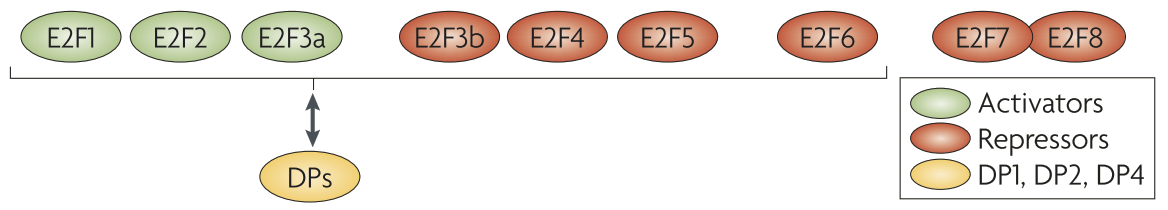
\includegraphics[width=0.9\textwidth]{pngs/E2F_family.png}
					\caption{The E2F family of transcription factors in mammals. {\footnotesize Adapted from \cite{VandenHeuvel2008}}}
					\label{fig:E2F_family}
				\end{figure}
				
				The most prominent regulator of Cyclin E in the canonical cell cycle is the transcription factor E2F1. It is a potent regulator of S phase entry and DNA synthesis.
				In \textit{Drosophila} endocycles, E2F1 is subject to regulation by the action of CRL4/Cdt2, an ubiquitin ligase that is activated upon DNA replication and thus itself a consequence of the E2F1 activity - a negative feedback mechanism \cite{Zielke2011}\cite{Havens2011}\cite{Shibutani2008}.  There is therefore an oscillation of E2F1 during endocycles that both promotes and is also the consequence of the oscillation of other key players in cell cycle regulation: 
				APC/C activity as a xXXXXXXXX is negatively regulated by Cyclin E-CDK2
				Cdt1 (essential replication licensing protein Cdt1 (Dup - droso))
				Gemini (inhibitor of Cdt1 - inhibited by APC)
				
				\begin{figure}[here]
					\centering
					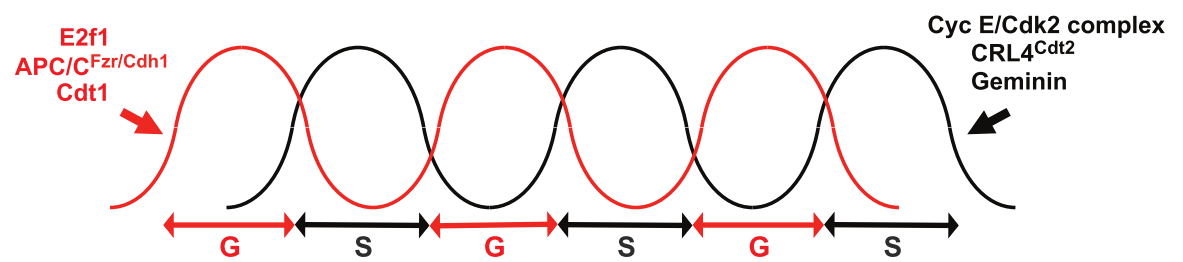
\includegraphics[width=0.9\textwidth]{pngs/oscilation.png}
					\caption{Oscillation of opposing networks of cell cycle genes during endocycles. {\footnotesize Adapted from \cite{Fox2013}}}
					\label{fig:oscillation}
				\end{figure}
				
				
				This is mechanism of regulation ensures DNA is replicated only once per S phase, and is consistent with the observation that E2F1 activity is necessary for 
				consistent 
			

			Nonetheless, these results emphasize that negative-feedback regulation is a common and important feature of molecular oscillators that control cell cycle progression (Ferrell et al., 2011). A central CDK oscillator provides a mechanism through which other important aspects of endoreplication can be controlled (Fig. 2). 
			For example, the oscillation of APC/C activity in Drosophila salivary glands probably results directly from the oscillation of Cyclin E/Cdk2 complex activity, which inhibits the APC/C (Narbonne-Reveau et al., 2008). Key targets of the APC/C during endoreplication progression are the mitotic cyclins and the protein Geminin, which is an inhibitor of the essential replication licensing protein Cdt1 (Dup – FlyBase).
			Indeed, the combination of mitotic Cdk1 inhibition and Geminin proteolysis can trigger endoreplication in human cells (Hochegger et al., 2007). By contrast, in Arabidopsis, little or no APC/C activity is required for endoreplication progression (as opposed to endoreplication entry, as described above), perhaps because there is no Geminin protein (Roodbarkelari et al., 2010). In Drosophila salivary glands, Geminin is absent during G phase, when replication licensing occurs, and present during S phase to prevent DNA licensing (Zielke et al., 2008).
			 In this way, the endoreplication S phase is similar to the S phase of a cell division cycle and distinct from the phenomenon of re-replication, in which specific segments of DNA are replicated more than once in a single S phase. In contrast to endoreplication, re-replication is an aberrant situation that causes genomic instability and is observed in some cancer cells (see Box 2).
			 In summary, the central endoreplication oscillator entrains many molecular activities to ensure the cycling of CDK activity and, thus, the cycling of replication licensing. It is important to keep in mind that the mechanism by which cyclic CDK activity is achieved may differ among species or even among different cell types within the same organism. For example, Drosophila nurse cells probably rely more on CKI activity than on E2F activity for CDK control during endoreplication (Hong et al., 2007). Nevertheless, the network of interactions controlling cyclic S phase CDK activity constitutes the central principle of endoreplication that we propose is universally applicable.

			Negative-feedback regulation of E2F activity is also important for endoreplication in hepatocytes (Chen et al., 2012; Pandit et al., 2012), but here it appears to control the transition from cell division to endoreplication, and it is not yet known whether E2F functions as part of a mammalian endoreplication oscillator.
			
			
			In another perspective, E2F7 is known to repress a network of cell cycle genes to control S-phase progression.\cite{Westendorp2012}
			\cite{Moon2008}
			\cite{Meserve2012}
			\cite{Chen2012}

	\section{Histone modifications in cell cycle regulation}
	The cell cycle is currently one of the most studied biological processes, due to its significance in growth and development and its deregulation in many human disorders. Studies using a diverse set of model organisms have greatly expanded knowledge of cell cycle regulation and have contributed to a uniform view of how the basic cell cycle machinery is regulated  \cite{Raynaud2014a}.
	
	Although studied for long, only recently have histone modifications been shown to contribute to it. This chapter of the review highlights the function of some post-translational histone modifications in cell cycle regulation.
		
		\subsection{The role of H2Bub in DNA replication}
		Monoubiquitylation of histone H2B on lysine 123 (H2Bub1) is known to be an important histone modification during transcription. H2Bub1 is promoted by the Bre1 ubiquitin ligase and this happens mainly in coding regions, particularly the ones that are being expressed. It is also a highly dynamic histone modification, with cycles of ubiquitylation and deubiquitylation naturaly occuring during the transcritpional process. I has been shown that this oscilation is required for proper transcriptional elongation through the control of the RNA Polymerase II (Pol II) and inhibition of recruitment of the CTK1 kinase, which has a function in later phases of transcription. H2Bub1 also controls the methylation state of both lysine 4 and 79 residues on histone H3 - two other important modifications in the transcriptional and replicative process \cite{Kouzarides2007}.
		
		The mechanistical similarities between transcription and replication suggest that H2Bub1 may have a role in replication as well. In both processes, nucleossomes must be displaced ahead of the replication fork and assembled again after (in replication in more strands than in the original template).
		
		In recent studies performed in the buddying yeast  \cite{Trujillo2012}, H2Bub1 has been shown to be enriched at replication origins, while the writer of this modification, Bre1, is also present. H2Bub1 continued to be present after replication, during G2 and M phases, suggesting that it is maintained on daughter strands of chromatin and after origins are fired for replication start.
		
		Hydroxyurea, a inhibitor of a ribonucleotide reductase enzyme required for deoxyribonucleotides production, has the effect of causing S phase arrest due to nucleotide depletion. When G1 arrested synchronized cells were released into hydroxyurea, Bre1 and H2Bub1 were detected at regions away from replication origins, posing the hypothesis that Bre1 could be travelling with the replissome as happens in transcription due to Pol II complex association \cite{Trujillo2012}.
		
		Using a mutant strain for H2BK123, it was possible to detect that H2Bub1 was shown to be not required for the initiation of DNA synthesis as mutant cells initiated DNA replication. Nevertheless, when accessed for their capability to complete replication in the same time as wild-type cells, H2BK123 mutants were slower, as accessed by the levels of H3K56ac and the G2/M marker Clb2. This confirmed the involvment of H2Bub1 in normal cell cycle progression, particularly in the elongation of DNA replication in S phase \cite{Trujillo2012}.
		
		Dissecting the reason of the inefficiency of H2BK123 mutant cells in replication elogation, it was shown that in these cell only a fraction of the factors required for replication elongation (Pol $\alpha$, Pol $\epsilon$ Mcm4, Cdc45 Psf2) did not accumulate significantly at positions downstream of replication origins when compared with wild-type cells. Additionaly, reduced intermediate single-stranded DNA was detected in mutants. Toghether this reveals the important role of H2Bub1 in the progression of replication forks, possibly through the interaction with other effectors necessary for replication elongation \cite{Trujillo2012}.
		
		In these mutant cells, it was also noted that global histone H3 levels were reduced in replication origins after replication compared with wild-type cells, pointing to either a defect in nucleossome assembly on newly synthesised strands or reduced stabilization of assembled nucleossomes \cite{Trujillo2012}.
		
		Spt16, a subunit of the FACT complex that is responsible for nucleossome displacement ahead of the transcription fork is known to interact with H2Bub1 to restore nucleossome ocupancy during elongation of transcription. In replication the same was also detected, with Spt16 present at replication origins and more distal positions with the replication fork advancement. However, in H2BK123 mutant cells, Spt16 was significantly reduced in distal replicating positions, suggesting that H2Bub1 stabilizes Spt15 on replicating chromatin \cite{Trujillo2012}.
		
		Taken together, evidence collected in this study \cite{Trujillo2012} showed an unprecedented role for a histone modification in replication. Ubiquitylation of H2BK123 is present in origins of replication, promotes efficient replication elongation and the stability of the replisome as well as nucleosome assembly or stability.
		
		\subsection{Dot1 and H3K79 methylation in the cell cycle}
	
		All known histone lysine methyltransferases contain a SET domain, with the exception of Dot1, which has a conserved catalytic core more similar to arginine methyltransferases. Dot1 is conserved from trypanosomes to humans and catalyses mono-, di- and trimethylation of histone H3K79, a residue located in the nucleosome core \cite{Kouzarides2007}. Until now, no protein has been identified that unambigously binds a specific methylated state of H3K79 or that can remove any methyl group from it \cite{Frederiks2008}.
		
		It has been shown that Dot1's mode of action is distributive \textit{in vivo} and not processive as all SET domain-containing methyltransferases \cite{Frederiks2008}. This means Dot1 acts in a ‘methylate-and-run’ fashion rather than using a multistep processive approach - this makes it the first known distributive protein lysine methyltransferase. This also implies that the initial methylation states of H3K79 are obligatory intermediates in the synthesis of higher methylation states by Dot1.
		
		The earliest known function of H3K79 methylation was in euchromatin, where it restricts Sir-mediated silencing of chromatin to regions of silent chromatin \cite{Frederiks2008}. In this function there is no correlation between the level of any of the specific methylation states and the degree of silencing, but the sum of all methylation states is indeed correlated, which implies that the different methylation states are likely to have redundant functions.
		
		It is also known that di- and trimethylation of H3K79 in yeast requires ubiquitination of histone H2B on Lys123 (H2Bub1) which is deposited by the Bre1 ubiquitin ligase. Bre1 does not specifically regulate H3K79 methylation but instead enhances its overall catalysis \cite{Kouzarides2007} \cite{Frederiks2008}. This has been proposed to be due to the possibility that the ubiquitin moiety directly affects the active site of Dot1 or that H2Bub1 affects the \textit{in vivo} chromatin substrate such that H3K79 on the nucleosome core becomes more accessible for interaction with Dot1 \cite{Frederiks2008}. The second option seems more supported due to the fact that \textit{in vitro}, H2BK123ub1 is not required for multiple methylation of H3K79 by Dot1.
		
		Dot1's distributive mode of action has prompted the mathematical modelling of H3K79 methylation states in yeast, using quantitative proteomics data, growth rates and estimates of nuclear Dot1 and histone abundance \textit{in vivo} \cite{DeVos2011}. This model predicts that increased states of H3K79 methylation accumulate with time until a H3K79me3-rich steady state is reached. Another important prediction is that each subsequent methylation reaction is slower than the one before - in agreement with a non-processive mechanism of methylation \cite{DeVos2011}.
			
		Since all states of H3K79 methylation accumulate during a cell's life cycle, one prediction of the model is that cell-cycle length can affect the average pattern of methylation throughout the cell cycle phases. This was confirmed experimentally with the observation that in slowly growing or arrested cells, H3K79 methylation is indeed higher, probably due to the fact that Dot1 has more time to introduce methyl groups. Over all cell cycle stages, it was noted a temporary drop in methylation during S phase, when new, unmodified histones are deposited on chromatin \cite{DeVos2011}. The level of H3K79me0 was highest in the S phase but progressive accumulation of methyl groups until a new S phase. This would implicate that H3K79 methylation is at least not fully maintained on new histones during replication. Nevertheless, only when the cell cycle time was doubled, a steady state of high H3K79me3 was reached, indicating that in a normal yeast cell cycle a steady state is not reached and histone renewal might play a role on the balance of H3K79 methylation \cite{DeVos2011}.
		
		The model thus accurately predicted the dynamics of H3K79 methylation through cell cycle and highlighted the importance of the residence time of histones in chromatin.	It was shown experimentally that the level of H3K79 methylation correlates with the age of the histones, regardless of the cell's age and that nucleossomes binding genes known for high histone turnover had significantly less H3K79 methylation. These observations confirm the temporal dependency between H3K79 methylation and the age of histones. The same dependency was not detected in H3K4 methylation, suggesting that the presence of a demethylase can counteract the accumulation of methylation on ageing histones \cite{DeVos2011}.
		
		This temporal dependence of H3K79 methylation has additional implications: epigenetic inheritance of H3K79 methylation states is hindered by the fact that at least one of the daughter cells will not receive the same information as the parent cell. This is incompatible with the current model of histone modification as marks of epigenetic memory. However it shouldn't be excluded that not the information of single nucleossomes, but the global state of H3K79 methylation over larger chromatin domains might bare epigenetic function.
		
		In \textit{Trypanossoma} - a unicellular eukaryotic parasite with considerable divergence of key cell cycle regulators - the view of H3K79 methylation (H3K76 in \textit{Trypanossoma}) as a carrier of epigenetic information is also challenged by the depletion of H3K79 methylation on newly incorporated histones during S phase \cite{Gassen2012}.
		
		In this organism there are two Dot1 homologue proteins of Dot1 (Dot1A and Dot1B) and there seems to be some division of labour between the two regarding the different methylation states of H3K79. Although both enzymes can mono- and dimethylate H3K79, Dot1A seems incapable of trymetylating H3K79, whereas Dot1B does, but it is not clear if both enzymes have the same affinity for the two shared methylation forms and therefore contribute equally \cite{Gassen2012}. Only Dot1A is required for survival.
	
		Depletion of Dot1A decreased H3K79 mono- and di-methylation and generated cells with reduced DNA content, which suggests a role for H3K79 methylation in accurate cell-cycle progression. These cells suffered complete replication inhibition which nevertheless didn't prevented cell division \cite{Gassen2012}.
		
		The inverse disturbance in Dot1A expression (overexpression) resulted in premature H3K79 methylation (during S phase) opposed to generalised increase of methylation levels. Nevertheless, this temporal deregulation caused continuous DNA replication which created cells with increased levels DNA content - the opposite effect of Dot1A depletion. This suggests that not only the global methylation states of H3K79 are implied in accurate cell cycle regulation, but that the timing of addition of this histone modification also plays a role at least in \textit{Trypanossoma} \cite{Gassen2012}.
		
		In human cells, depletion of Dot1, and consequently H3K79 methylation, did not seem to affect replication mechanism itself since the frequency of replication initiation events, replication fork velocity and the proportion of cell cycle phases were not different when compared with normal cells \cite{Fu2013a}. However, an increased fraction of cells exhibiting DNA content greater than 4N and apoptosis was detected.
		
		Although cells were still able to proliferate and replicate DNA in the absence of H3K79 methylation, its absence affected the regulatory processess modulating the timing of DNA replication, for the causes of a higher fraction of cells with higher ploidy than normally were identified as cells skipping mitosis after S phase and re-replicating their DNA without completing cell division \cite{Fu2013a}.
		
		This deregulation of replication timing led to the hypothesis that Dot1 mediated H3K79 methylation marks origins of replication that have started replication, preventing replication initiation a second time before the cell completes division. In the case of cells lacking Dot1, the cause of re-replication might then be new replication from origins or replication that had already been used previously in the same cell cycle. This hypothesis is supported by evidence that H3K79me2 was shown to be associated with functional replication origins, but not with a mutant replication origin that resembled a functional one \cite{Fu2013a}.
		
		These studies highlight the non-canonical use of a histone modification (H3K79 methylation) and show its importance in the regulation of replication, a major cellular event.

	%%%%%%%%%%%%%%%%%	
	
	\section{\textit{Oikopleura dioica}, a cross-disciplinary model system}
		\textit{Oikopleura dioica} is a marine chordate organism belonging to the class Appendicularia, which is a member of the Tunicate subphylum along with the classes Thaliacea (salps) and Ascidiacea (sea squirts). Tunicates are the most closely extant group related to the vertebrates (see Figure ~\ref{fig:tree}). \textit{Oikopleura} shares some biological traits with most tunicates (\textit{e.g.} filter feeding), but unlike them has some peculiarities which make it a very interesting model for the study of many biological features. \textit{Oikopleura dioica} owes its name to the fact that it is the only dioeicious appendicularian known, being most other species hermaphrodites.
		
		\begin{figure}[here]
			\centering
			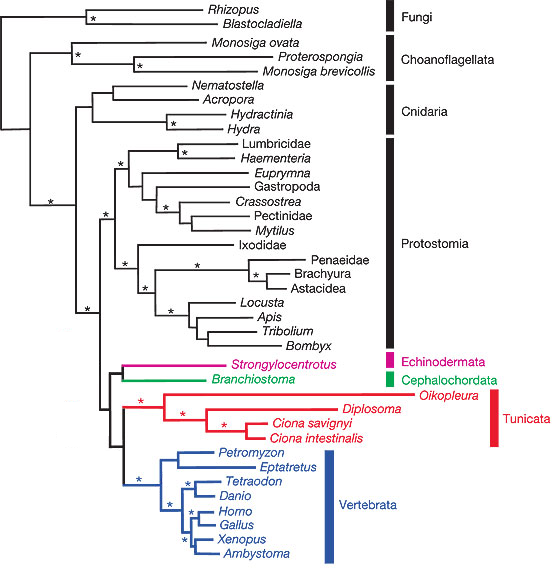
\includegraphics[width=0.5\textwidth]{tree.jpg}
			\caption{Phylogeny of the Deuterostome group with emphasis on the Tunicate subphylum}
			\label{fig:tree}
		\end{figure}
		
		\subsection{	\textit{Oikopleura}'s life cycle}
		\textit{Oikopleura} reproduces through external fertilization after the rupture of both female and male gonads or sperm release via the spermiduct \cite{}. The first cell division remarkably occurs only 35 min after fertilization and a XXXXXXX gastrulation takes place after two hours when at 20ºC. Four hours after fertilization the animal is ventrally bent with on its tail (Tailbud stage) and later hatches from the chorion to be a free-swimming larva. Figure \ref{fig:LifeCycle} represents the early development of \textit{Oikopleura}.
		
		Larval development takes place until fifteen hours after fertilization, where a metamorphosis known as Tailshift occurs and the tails changes orientation towards the ventral side of the animal. At this point, most cells stop mitotic division and start performing endocycling, a endoreduplicative cell division strategy which gives rise to multinucleated cells and increases body size by increasing the cell volume (discussed in detail in Section \ref{subsection:CellCycleVariants}). This strategy continues throughout most of the remaining juvenile life of \textit{Oikopleura} until the third day of development, where gametogenesis starts in the rapidly growing gonad. Most of \textit{Oikopleura}'s growth until the end of its life at day six is dedicated to gonad maturation, which at its peak reaches a total volume bigger than the somatic part of the whole organism. This is achieved again through the employment of endocycling in the gonad.
		
		\begin{figure}[here]
			\centering
			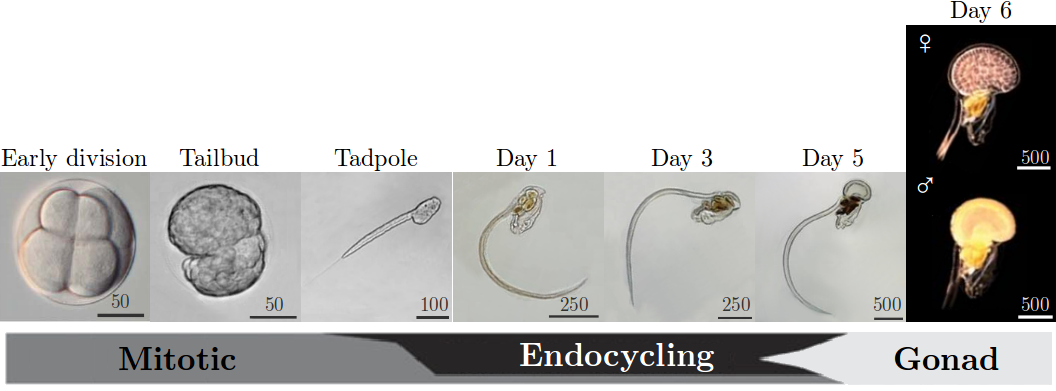
\includegraphics[width=0.5\textwidth]{lifeCycle.jpg}
			\caption{Diagram of \textit{Oikopleura dioica}'s development through its life cycle}
			\label{fig:LifeCycle}
		\end{figure}
		

		\subsection{The genome of \textit{Oikopleura dioica}}
		\textit{Oikopleura} reference genome sequence was made available in 2010 \cite{}, revealing a surprisingly plastic architecture and the species fast evolution.

		% compact
		In this planctonic animal, the chordate genome architecture seems to have been redesigned to obtain a minimal-sized genome: approximately 70 megabases. This is greatly due to the reduction of intron and intergenic space, although some gene loss also could also be detected. The dramatic reduction of intergenic space brings obvious constrains in terms of gene regulation, which is to some degree easily seen by the normal occurrence of genes in Operons (~28\% of the 18000 total), but makes the \textit{Oikopleura} genome one of the most compact of all known chordate genomes.
		Operons are significantly enriched for genes involved in house-keeping functions, while genes involved in developmental processes are significantly under-represented in Operons.
		Although a generalised change in cis regulatory modules seems a plausible hypothesis, cis regulation seems to take place. Highly Conserved Elements have been found through genomic alignments between Atlantic and Pacific \textit{Oikopleura dioica}.
		
		Nevertheless, several conserved genomic features can be found in the \textit{Oikopleura} genome.
		Long introns are more likely to be old than are short ones.
		Developmental genes show a double proportion of old introns compared to all annotated genes.
		
		
		\subsection{Histone variants in \textit{Oikopleura dioica}}
		\cite{Moosmann2011}

canonical core histones:
	replication dependent (RD) genes
	lack introns
	organized in gene clusters
	mRNAs possess a conserved stem-loop (SL) in the 3’UTR coupling gene expression to DNA replication

histone variants:
	are often transcribed from orphan genes
	contain introns
	lack the SL and their expression is not restricted to S-phase
	they are referred to as replacement or replication-independent (RI) variants.

H4 is highly constrained as it contacts with the other 3 core histones and its N-terminal tail residues are subject to extensive PTMs.
			
		\subsection{CDK repertoire of \textit{Oikopleura dioica}}
		
		\subsection{Cell cycle variants in \textit{Oikopleura dioica}}
		\label{subsection:CellCycleVariants}
		O. dioica displays an unique system of cell cycle regulation that is poorly understood, because previous research on cell cycle have focussed on a single nuclei within its own cytoplasm, while in this model we can study cell cycle regulation of multiple nuclei, both meiotic and endocycling, sharing a common cytoplasm, as seen in the coenocyst. Cell cycle in O. dioica is also unique in its way of development because most cells switch from rapid mitotic division to endoreduplication around the event of tail shift. O. dioica is also an important organism when viewed at the light of evolution, because it is the closest evolutionary relative to the vertebrates, and is therefore an important model organism in the field biology. In addition to presenting a unique environment for cell cycle studies and its evolutionary importance, it has many other abilities that make it an excellent model organism. O. dioica is successfully maintained in culture and have a short life cycle of 6 days at 15°C (Bouquet, 2009), and is therefore an excellent model organism for developmental studies. It is also transparent which makes it easy to observe internal organs when used for in situ experiments. Another advantage of using O. dioica as a model organism is the fact that the genome of O. dioica has been fully sequenced, which makes genetic studies easier by far.
		
		
		\subsubsection{Endocycling}
	
	
	\section{Project Goals}
		Identify the roles of the Oikopleura E2F TF family in endocycles
		Gain insights on the epigenetics basis for endocycle regulation mediated by H3K79me and it's methyltransferase Dot1L

\clearpage

%=========================================================================%
\chapter{Materials and Methods}
%=========================================================================%
	\section{Materials}
		\subsection{Antibodies}
			\begin{table}[H]
       		\caption{\bf{Antibodies used for ChIP, immunofluorescence and western blot}}
        		\begin{center}
            		\begin{tabular}{p{2cm} | p{8cm} | p{3cm} | p{3cm}}
	                	\textbf{Antibody} & \textbf{Description} & \textbf{Supplier} & \textbf{Purpose}\\
    		            \hline
        		        ab46540 & Rabbit Control IgG - ChIP Grade & Abcam & ChIP\\
            		    ab & RNA Polymerase II CTD & Abcam & ChIP\\
            		     & E2F1 & & ChIP\\
						 & E2F7 & & ChIP\\
            		    ab10543 & Anti-Histone H3 (phospho S28) [HTA28] & Abcam & Immunostaining\\
            		    39143  & Anti-Histone H3 K79me2 Rabbit & Active Motif & Immunostaining and Western blot\\
            		    05-1312  &  Anti-Ubiquityl-Histone H2B Mouse & Milipore & Immunostaining\\
            		    \hline
            		    A-21206 & Anti-Rabbit IgG secondary antibody conjugated with Alexa 488 fluorochrome &  Molecular Probes & Immunostaining\\
               		    & Anti-Mouse IgG secondary antibody conjugated with Alexa 488  fluorochrome &  & Immunostaining\\
            		    & Anti-Rat IgG secondary antibody conjugated with Alexa 568 fluorochrome & & Immunostaining\\
            		    & Anti-Rabbit IgG secondary antibody conjugated with horseradish peroxidase &  & Western blot\\
	            	\end{tabular}
    		    \end{center}
		    \end{table}
		  
		\subsection{Chemicals and reagents}
		
			\begin{table}[H]
       		\caption{\bf{Chemicals and reagents used in various protocols}}
        		\begin{center}
            		\begin{tabular}{c|c|c}
	               		Supplier & Chemical & Purpose\\
    		            \hline
    		            Thermo Scientific & 16\% Formaldehyde Ampoules, Methanol-free & ChIP\\
    		            Tocris Bioscience & SGC0946 & H3K79me studies\\
	            	\end{tabular}
    		    \end{center}
		    \end{table}
    
	    \subsection{Consumables}
	    \label{subsection:consumables}
			\begin{table}[H]
       			\caption{\bf{Consumables with particular relevance in certain protocols}}
        		\begin{center}
            		\begin{tabular}{p{2.9cm} | p{8.2cm} | p{2.2cm}}
	                	\textbf{Supplier} & \textbf{Consumable} &  \textbf{Purpose}\\
    		            \hline
    		            Sigma-Aldrich & BD Precisionglide syringe needles - gauge 27, L 1/2 inches & ChIP\\
    		            Covaris & AFA microtubes & ChIP\\
						Sigma-Aldrich & Siliconized microtubes 1.7 mL capacity & ChIP\\
        		        Invitrogen & Protein G magnetic beads & ChIP\\
        		        Life Technologies & Qubit dsDNA HS assay kit & ChIP\\
        		        Bio-Rad & Mini-PROTEAN TGX stain-free gel & Western blot\\
        		        Bio-Rad & Trans-Blot turbo mini nitrocellulose membrane & Western blot\\
						Bio-Rad & Precision Protein StrepTactin-HRP Conjugate & Western blot\\
        		        Bio-Rad & Clarity western ECL substrate & Western blot\\
        		        Molecular Probes & TO-PRO-3 Iodide stain & Immunostaining\\
	            	\end{tabular}
    		    \end{center}
		    \end{table}
    
    		\subsection{Instruments and equipment}
			\begin{table}[H]
       		\caption{\bf{Instruments with particular relevance in certain protocols}}
        		\begin{center}
            		\begin{tabular}{p{3.1cm} | p{8.5cm} | p{2.2cm}}
	               		\textbf{Supplier} & \textbf{Instrument/equipment} & \textbf{Purpose}\\
    		            \hline
						Covaris & S200 focused sonicator & ChIP\\
						Thermo Scientific & Nanodrop ND-1000 spectrophotometer & ChIP\\
						Life Technologies & Qubit 2.0 fluorometer & ChIP\\
						BioRad & C1000 thermocycler with CFX96 module & ChIP\\
						Leica & TCS-SP5 confocal microscope with Ar-Kr ion laser & Microscopy\\
						Bio-Rad & Trans-Blot turbo transfer system & Western blot\\
						Bio-Rad & ChemiDox XRS imaging system & Western blot\\
	            	\end{tabular}
    		    \end{center}
		    \end{table}
		    
		\subsection{Buffers and solutions}
			\subsubsection{ChIP}
				\begin{description}
					\footnotesize
					\item[PBS, pH 7.4] 1.37 M NaCl, 27mM KCl,100 mM Na2HPO4, 1.8 mM KH2PO4
					\item[Lysis buffer] 150mM NaCl, 1\% NP-40, 0.5\% Na deoxycholate, 0.1\% SDS, 50 mM Tris pH 8, 1mM EDTA					
					\item[PBS-T] 0.02\% Tween-20 in PBS
					\item[Lithium chloride buffer] 50 mM Tris pH 8, 250mM LiCl, 0.5\% NP-40, 0.5\% Na deoxycholate
					\item[TE buffer] 10 mM Tris pH 8, 1 mM EDTA
					\item[Elution buffer] 50 mM Tris pH 8, 1 mM EDTA, 0.1\% SDS
				\end{description}
				
		    \subsubsection{Western blot}
		    \label{subsection:Westernbuffers}
				\begin{description}
					\footnotesize
					\item[Laemmli extract] 200 mM Tris-HCl pH 6.8, 8\% SDS, 40\% glycerol, 0.004\%bromophenol blue (400 mM 2-mercaptoethanol - added fresh)
					\item[Polyacrilamide gel, stacking portion] 6\% bis-acrilamide, 125 mM Tris pH 6.8, 0.1 \%SDS, 0.1\% ammonium persulphate,  0.1\% TEMED
					\item[Polyacrilamide gel, running portion] 8-18\% bis-acrilamide, 370 mM Tris pH 8.8, 0.1 \%SDS, 0.1\% ammonium persulphate,  0.1\% TEMED
					\item[SDS-PAGE running buffer] 25 mM Tris, 192 mM glycine, 0.1\% SDS
					\item[TBS, pH 7.4] 1.5M NaCl, 0.2M Tris
					\item[TBS-T] 1.5M NaCl, 0.2M Tris, 0.1\% Tween-20
					\item[PBS, pH 7.4] 1.37 M NaCl, 27mM KCl,100 mM Na2HPO4, 1.8 mM KH2PO4
					\item[Transfer buffer] 25 mM Tris, 192 mM glycine (10\% methanol - added fresh)
					\item[Ponceau S stain] 2\% Ponceau S, 30\% trichloroacetic acid, 30\% sulfosalicylic acid
				\end{description}
			
			\subsubsection{Immunostaining}
			     \begin{description}
					\footnotesize
					\item[Fixative] 4\% paraformaldehyde, 100 mM MOPS pH 7.5, 500 mM NaCl
					\item[PBS, pH 7.4] 1.37 M NaCl, 27mM KCl,100 mM Na2HPO4, 1.8 mM KH2PO4
					\item[PBS-T] 0.02\% Tween-20 in PBS buffer
					\item[PBS-TE] 0.02\% Tween-20, 1 mM EDTA in PBS buffer
					\item[PBS-TEG] 0.02\% Tween-20, 1 mM EDTA, 100 mM glycine in PBS buffer
					\item[Blocking solution] 3 \% acetylated bovine serum albumin (BSA) in PBS-TE buffer
				\end{description}
		    		    
		    
	\section{Animal culture and collection}
		\subsection{Culture of \textit{O. dioica}}
		The culture of \textit{Oikopleura} was performed at the SARS centre appendiculatian facility as previously described \cite{Bouquet2009}. Cultured animals are native from the coastal area outside Bergen and are frequently collected and added to the permanent culture. Animals are permanently cultured at the facility in 6L seawater beakers, with permanent stirring and daily water renewal as well as feeding twice daily with algae according to the developmental stage (see table \ref{table:ODculture}). The use of a fixed volume for culture implies the progressive dilution of animals until the third day of life, where density remains at 150 animals per 6L beaker.
		
		\begin{table}
       		\caption{\bf{Feeding regime of \textit{Oikopleura} according to developmental stage}}
       			\begin{center}
            		\begin{tabular}{ c | c | >{\centering\arraybackslash}m{1.6cm}  | >{\centering\arraybackslash}m{2.1cm}  | >{\centering\arraybackslash}m{2.0cm} | >{\centering\arraybackslash}m{2.2cm} | >{\centering\arraybackslash}m{1.8cm} }
		                \multicolumn{2}{c|}{} & \small{\textbf{\textit{Isochrysis sp.}}} & \small{\textbf{\textit{Chaetoceros calcitrans}}} & \small{\textbf{\textit{Rhinomonas reticulata}}} & \small{\textbf{\textit{Synecococcus sp.}}} & \small{\textbf{Crushed \textit{R. reticulata}}}\\
        		        \multicolumn{2}{c}{\small{Development time}} & \multicolumn{3}{|c|}{(cells/mL)} & \multicolumn{2}{c}{(mL)} \\
        		        												 \hline
        		        \multirow{2}{*}{1} 	& Morning & 2000 & 2000 & 0 & 5 & 5\\
        		        												& Evening & 1000 & 1000 & 0 & 3 & 5\\
        		        												 \hline
        		        \multirow{2}{*}{2} 	& Morning & 2000 & 2000 & 0 & 5 & 5\\
        		        												& Evening & 1000 & 1000 & 0 & 3 & 5\\
        		        												 \hline
        		        \multirow{2}{*}{3} 	& Morning & 2000 & 4000 & 0 & 5 & 5\\
        		        												& Evening & 1000 & 2000 & 1000 & 3 & 5\\
        		        												 \hline
        		        \multirow{2}{*}{4} 	& Morning & 4000 & 4000 & 2000 & 0 & 5\\
        		        												& Evening & 2000 & 2000 & 1000 & 0 & 5\\
        		        												 \hline
        		        \multirow{2}{*}{5} 	& Morning & 4000 & 4000 & 2000 & 0 & 5\\
        		        												& Evening & 2000 & 2000 & 1000 & 0 & 5\\
	           			\end{tabular}
       				\end{center}
        		\label{table:ODculture}
		    \end{table}
		
		\subsection{Collection of \textit{O. dioica}}
			\subsubsection{Tailbud stage}
			To collect \textit{Oikopleura} in the Tailbud developmental stage, a controlled \textit{in vitro} fertilization was performed. Day six mature male animals were collected to a Petri dish with seawater and allowed to spawn. When all male animals had spawned, sperm quality was visually inspected on a light microscope for motility. Day six mature females were individually collected to glass salliers with seawater and allowed to spawn at 18ºC. When spawned, 60$\mu$L of sperm solution was added to the sallier and after 3-4 hours tailbud animals collected to a eppendorf microtube.
			
			\subsubsection{Day two stage}
			Late day two \textit{Oikopleura} were individually collected with the aid of a 2 mL plastic pipette to a 1 L beaker with clean seawater (no algae) and stayed there 3 to 4 hours to be allowed to empty the gut of any remaining algae as well as build a new clean house.
			To achieve release of the houses, animals were individually collected again, this time using a mouth-pipette built from a 1 mL plastic pipette and poured into a glass recipient on ice with 0.125 mg/mL MS222 and allowed to sink to the bottom, where a third collection using a 200 $\mu$
			L micropipette took them to a 1.5 mL microtube.
			
			\subsubsection{Day six, immature stage}
			Immature day six animals with a visible gonad but naked-eye indistinguishable features were collected from culture into a 500 mL plastic beaker with clean seawater with the aid of a 25 mL plastic pipette and from there to a 1.5 mL microtube with a 2 mL plastic pipette. 
		
	
	\section{ChIP-seq}
		\subsection{Animal fixation}
			Tailbud and day two animals were briefly spin at 5000 g for 10 seconds to be collected at the bottom of the microtube, while day six immature voluntarily sank in seconds time. Seawater was exchanged for 0,5 mL PBS and 0,5 ml of either 1 or 2\% Formaldehyde in PBS was added to have a final fixative concentration of 0.5 or 1\% respectively, and let rotating for a variable amount of time as shown in Table \ref{table:ODfixation}, depending of the developmental stage. %Use good quality, methanol-free formaldehyde (see materials) and always opened fresh.
			
			Formaldehyde was quenched with Glycine solution to stop fixation and again let rotating for 5 min at 18ºC. 
			Again by either spinning at 5000 g for 30 seconds or allowing animals to freely sink, Formaldehyde was removed and animals washed with cold PBSplus three times on ice, after which all solution was removed and animal pellets frozen with liquid nitrogen and stored at -80ºC for future use.
    
    		 \begin{table}[!ht]
	    	    \caption{\bf{Fixation conditions for each tested developmental stage of \textit{Oikopleura dioica}}}
        		\begin{center}
		            \begin{tabular}{c|c|c|c}
                		\textbf{Stage} & \textbf{Fixative concentration} & \textbf{Time (min)} & \textbf{Temperature (ºC)}\\
		                \hline
		                Tailbud & 1\% & 5 & 18\\
		                Day two & 0.5\% & 5 & 18\\
		                Day six immature & 1\% & 10 & 18\\
        		    \end{tabular}
		        \end{center}
        		\label{table:ODfixation}
		    \end{table}
    
    			\subsection{Cell lysis and chromatin sonication}
			Frozen animals pellets were thawed on ice and pooled with the aid of cold Lysis buffer to a total volume multiple of 130$\mu$L but never less than 390$\mu$L depending on the total amount of animal material.		
			Mechanical lysis was conducted with a 27-gauge XXXXXX needle and 2 mL syringe passing the whole volume no less than three times through the needle and incubated on ice 15 min.
			
			Sonication was performed on a S200 Covaris focused sonicator on a 4ºC water bath with 130$\mu$L AFA glass microtubes. The instrument settings used to sonicate the chromatin to a approximate gaussian distribution within 100-800 bp can be seen on Table \ref{table:CovarisSettings}. \\
			Whole sonicated lysates were centrifuged for 10 min, at 21000 g at 4°C and the chromatin-enriched supernatant was collect to a siliconized microtube.
			
			\begin{table}[!ht]
        		\caption{\bf{Settings used on the S200 Covaris sonicator for \textit{Oikopleura dioica} chromatin}}
        		\begin{center}
	        		\begin{tabular}{l|c}
		           		\textbf{Setting} & \textbf{Value}\\
	        		    \hline
		        		Duty cycle& 5\%\\
	            	    Intensity & 7.5\\
						Processing time & 5 minutes\\
		        		Bath temperature & 5-6 ºC\\
						Power mode & Frequency sweeping\\
		        		Degassing mode & Continuous\\
		        		Volume & 130 $\mu$L\\
		        		AFA intensifer & Integrated\\
	        			Water level & 8\\
	        		\end{tabular}
    		    \end{center}
	        \label{table:CovarisSettings}
		    \end{table}
			
			\subsection{Chromatin quality assessment}
			\label{section:chromQualityAssess}
			Total protein yield of chromatin was quantified with the Bradford assay with a 30:1 ratio of Coomassie reagent to chromatin and measured on a Nanodrop instrument.
			
			To check the distribution of the sonicated chromatin fragments, 1\% SDS, 100mM NaCl and 50 $\mu$g/mL RNAse A were added to a fraction of the chromatin and incubated for 30 min at 55ºC. Proteinase K was added to 200 $\mu$g/mL and samples incubated 90 min to O/N at 65ºC to reverse crosslinks. DNA was purified with the Phenol-Chloroform method and precipitation with ethanol. Briefly, an equal volume of Phenol:Chloroform:Isoamyl Alcohol (25:24:1) was mixed to the samples, and after centrifugation the 30 $\mu$g Glycogen, 300 mM Sodium Acetate and cold 70\% Ethanol (final concentrations) were added to the aqueous phase in a new microtube and incubated at -80ºC for 1 hour. After centrifugation at 4ºC, DNA pellets were washed with 70ºC Ethanol and dissolved in 3 to 5 $\mu$L TE buffer. \\
			
			DNA quality and amount was quantified on a Nanodrop instrument and loaded on an Agilent DNA High Sensitivity digital electrophoresis chip, to assess the distribution of DNA fragments with an Agilent Bioanalyzer instrument.
			
			\subsection{Immunoprecipitation}
			Protein G magnetic beads were washed once with PBS-T in siliconized tubes, incubated at 4ºC rotating for two hours with 10 $\mu$g of antibody and washed again with PBS-T and Lysis buffer.
			
			800 $\mu$g of chromatin were added to the magnetic beads with the already bound antibody and left O/N rotating at 4ºC, after which a series of 15 min, 4ºC washes followed: three with Lysis buffer without any inhibitors; two with Lithium chloride buffer; one with TE buffer.
			
			Elution of IP-enriched DNA followed with the addition of elution buffer and incubation at 65ºC for 15 min horizontally stirring at 900 rpm. A second, more stringent elution was performed with TE buffer with 500 mM NaCl and both supernatants were pooled.
			
			Reversal of crosslink took place during a three to five hour incubation at 65ºC, after which 50 $\mu$g/mL RNAse A were added, incubated at R/T for 10 min, and incubated again this time with 200 $\mu$g/mL Proteinase K at 55ºC O/N. Phenol-Chloroform extraction followed as previously described on section \ref{section:chromQualityAssess}, with the exception of final pellet dilution in 50 $\mu$L TE buffer.
			
			1 $\mu$L of sample was used in a Qubit high-sensitivity assay to measure total dsDNA yield from the ChIP assay.
			
			\subsection{qPCR}
			Enrichment of the ChIP samples was assessed through quantitative polymerase chain reaction (qPCR). PCR reactions were performed with 5 $\mu$L DNA from  either the ChIP sample or IgG control and the same set of primers amplifying regions of interest with 80-120 bp total length (see appendix \ref{appendixQPCRprimers}).
			
			Enrichments were calculated as XXXXXXXXXXXX
		
			\subsection{Illumina library construction and high-throughput sequencing}
			ChIP libraries were made using the Ovation Ultralow Library kit according to the manufacturer. Selected DNA fragments were within 150-350 bp and each set of biological replicates (16 samples) was sequenced in a single lane of a Illumina HiSeq 2500 instrument with 100 bp paired-end reads in Ohio, USA.
		
	\section{Western blot}
			\subsection{Sample preparation}
			Animals of the required stage were collected in microtubes and washed once with PBS. Laemmli buffer with fresh 2-mercaptoethanol was added to a final 1x concentration and samples were boiled at 99ºC for 10 minutes with mild agitation. After a 5 minute centrifugation at 16000 g , samples were snap frozen in liquid nitrogen and stored at -20ºC for later use.
			
			\subsection{SDS-PAGE}
			SDS-polyacrylamide gel electrophoresis was performed using either precast or self-casted gels (see section \ref{subsection:consumables} or \ref{subsection:Westernbuffers} respectively). The total volume of samples, as well as 8$\mu$L of protein marker were loaded and gels were run for 20 minutes at 50 V and then approximately 90 minutes at 150 V in running buffer.
			
			\subsection{Protein transference}
			Electrophoretically separed proteins were transfered to a nitrocelulose membrane using the a semi-dry transfer system with a program optimized for low molecular weight proteins (5 minutes transfer at XXXXX V).
			
			The nitrocellulose membrane was washed once in TBS buffer for 10 minutes, incubated in 1:10 Ponceau stain in TBS for 5 minutes and briefly rinsed with distilled water to allow visualization of protein, and an assessment of the transference efficiency. Ponceau stain was removed with two TBS-T washes.
			\subsection{Blotting}
			To reduce unspecific antibody binding, the membrane was blocked with 5\% fat-free milk or 3\% BSA in TBS-T for 60 minutes at R/T with mild horizontal shaking.
			
			The membrane was incubated with primary antibody dilluted 1:500 in 5\% fat-free milk O/N at 4ºC, and washed for 10 minutes at R/T with mild horizontally shaking, once with TBS, twice with TBS-T and again with TBS.
			
			Secondary antibody incubation diluted 1:5000 in 5\% fat-free milk was added to the membrane and this incubated for one hour at R/T toghether with 1:5000 WesternC XXXXXXX -HSP . Following washed were as after primary antibody incubation: 10 minutes at R/T with mild horizontally shaking, once with TBS, twice with TBS-T and again with TBS.
			\subsection{Detection}
			The membrane was washed once with PBS and incubated for 5 minutes in ECL substrate to allow detection of secondary antibody binding through chemiluminescence, being scanned with an exposure time between 3 and 30 seconds depending on signal strength.
		
	\section{Whole mount immunostaining}
		Collected animals were fixed in 4\% paraformaldehyde at 4ºC overnight and washed once with PBS-TE and twice with PBS-TEG to quench remaining formaldehyde. Two TBS-TE washes followed, after which animals were inculated O/N in blocking solution.
		
		Primary antibodies were diluted 1:100 in blocking solution and added to the animals after the previous blocking solution was removed from the microtubes. An incubation of at least six days with the primary antibodies was performed at 4ºC
		
		After primary antibody binding, six PBS-TE washes in 10 min intervals followed to remove any unbound primary antibody traces. A post-fixation similar to the primary one followed: 4\% formaldehyde in PBS-TE was added, and fixation took place O/N at 4ºC, after which one wash with PBS-TE and two with PBS-TEG followed. 
		
		Secondary antibodies diluted 1:500 in blocking solution were added to the animals  and these were left for another minimum of six days at 4ºC in darkness, to allow antibody binding and avoid weakening of fluorescent signal. Another six washes of PBS-TE followed, with the particularity that ToPRo3 was added to the fourth wash, diluted 1:1000, therefore allowing DNA staining.
		
		Animals were mounted in glass slides with Vectashield and imaged with confocal microscopy.
		
	\section{Data analysis}
		\subsection{QC, mapping}
		\subsection{E2F peak-finding}
		\subsection{E2F target-gene association}
		\subsection{E2F target-gene GO}
		\subsection{H3K79me domain identification}
		\subsection{pre-post Dot1L inhibition diferences on H3K79me and GO of genes involved}

	\section{Dot1L inhibition and knockout}
		\subsection{Inhibitor incubation}
		\subsection{Microinjections}


\clearpage


%=========================================================================%
\chapter{Results}
%=========================================================================%

\section{E2F factors in \textit{Oikopleura}'s late developmental stages}

	E2F expression in Figure \ref{fig:E2F_expression}
	
	\begin{figure}[here]
		\centering
		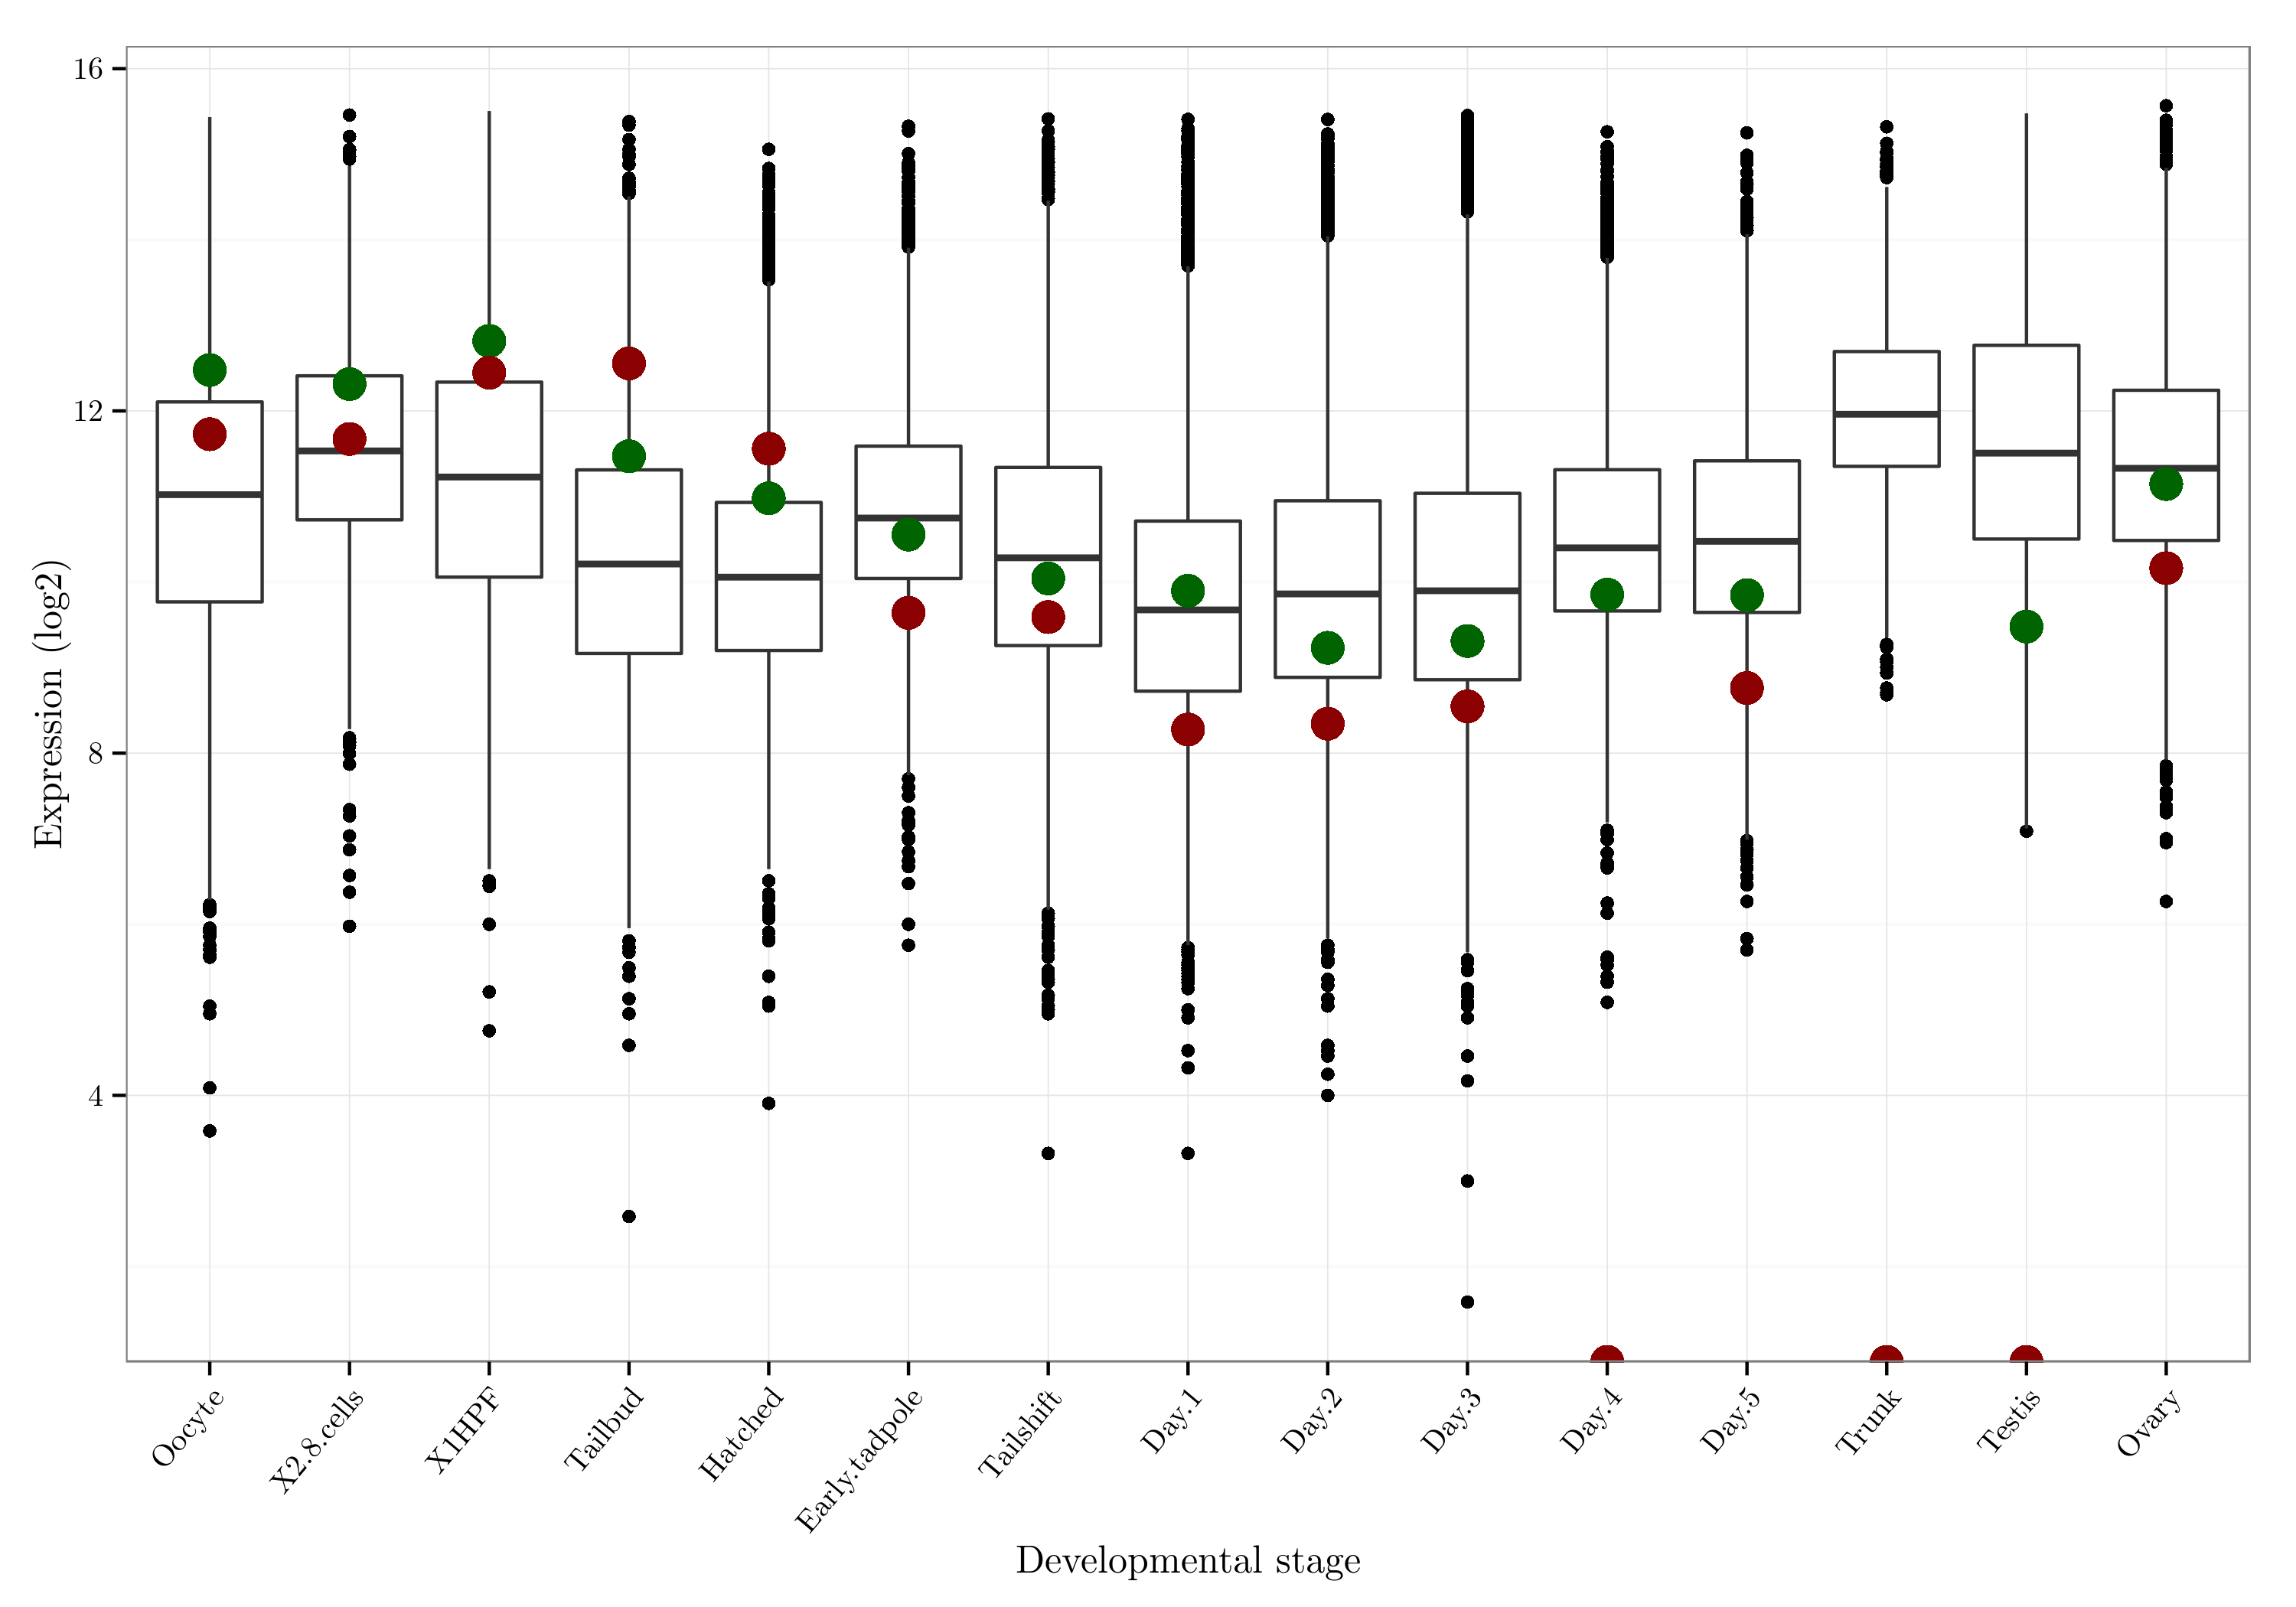
\includegraphics[width=0.9\textwidth]{pngs/E2F_expression_+allgenes.png}
		\caption{Expression of E2F factors during \textit{Oikopleura dioica}'s development.
			{
				\footnotesize
					Green: E2F1;
					Red: E2F7;
					Boxplots: All genes.
					Expression values transformed with a logarithm of base 2.
			}
		}
		\label{fig:E2F_expression}
	\end{figure}

	\subsection{E2F binding}
	
		Oikopleura's genome is compact, with reduced intergenic and intronic space, and enlarged proportion of coding sequence (Figure \ref{fig:genome_background}).
	
		\begin{figure}[here]
			\centering
			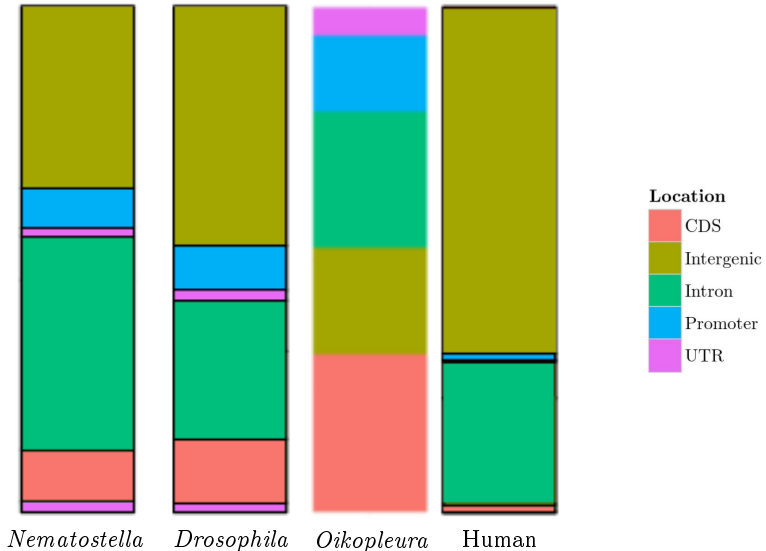
\includegraphics[height=0.5\textwidth]{pngs/species_genome.png}
			\caption{Comparison of the relative distribution of genomic locations in \textit{Oikopleura dioica} and other animal models. {\footnotesize From left to right: \textit{Nematostella vectensis}, \textit{Drosophila melanogaster}, \textit{Oikopleura dioica}, \textit{Homo sapiens}} }
			\label{fig:genome_background}
		\end{figure}
		
		E2F ChIP-ER locate near genes transcription start sites (TSS) (Figure \ref{fig:distance_to_TSS}).
		
		\begin{figure}[here]
			\setlength{\belowcaptionskip}{5pt}
			\centering
			\begin{subfigure}[b]{0.75\textwidth}
				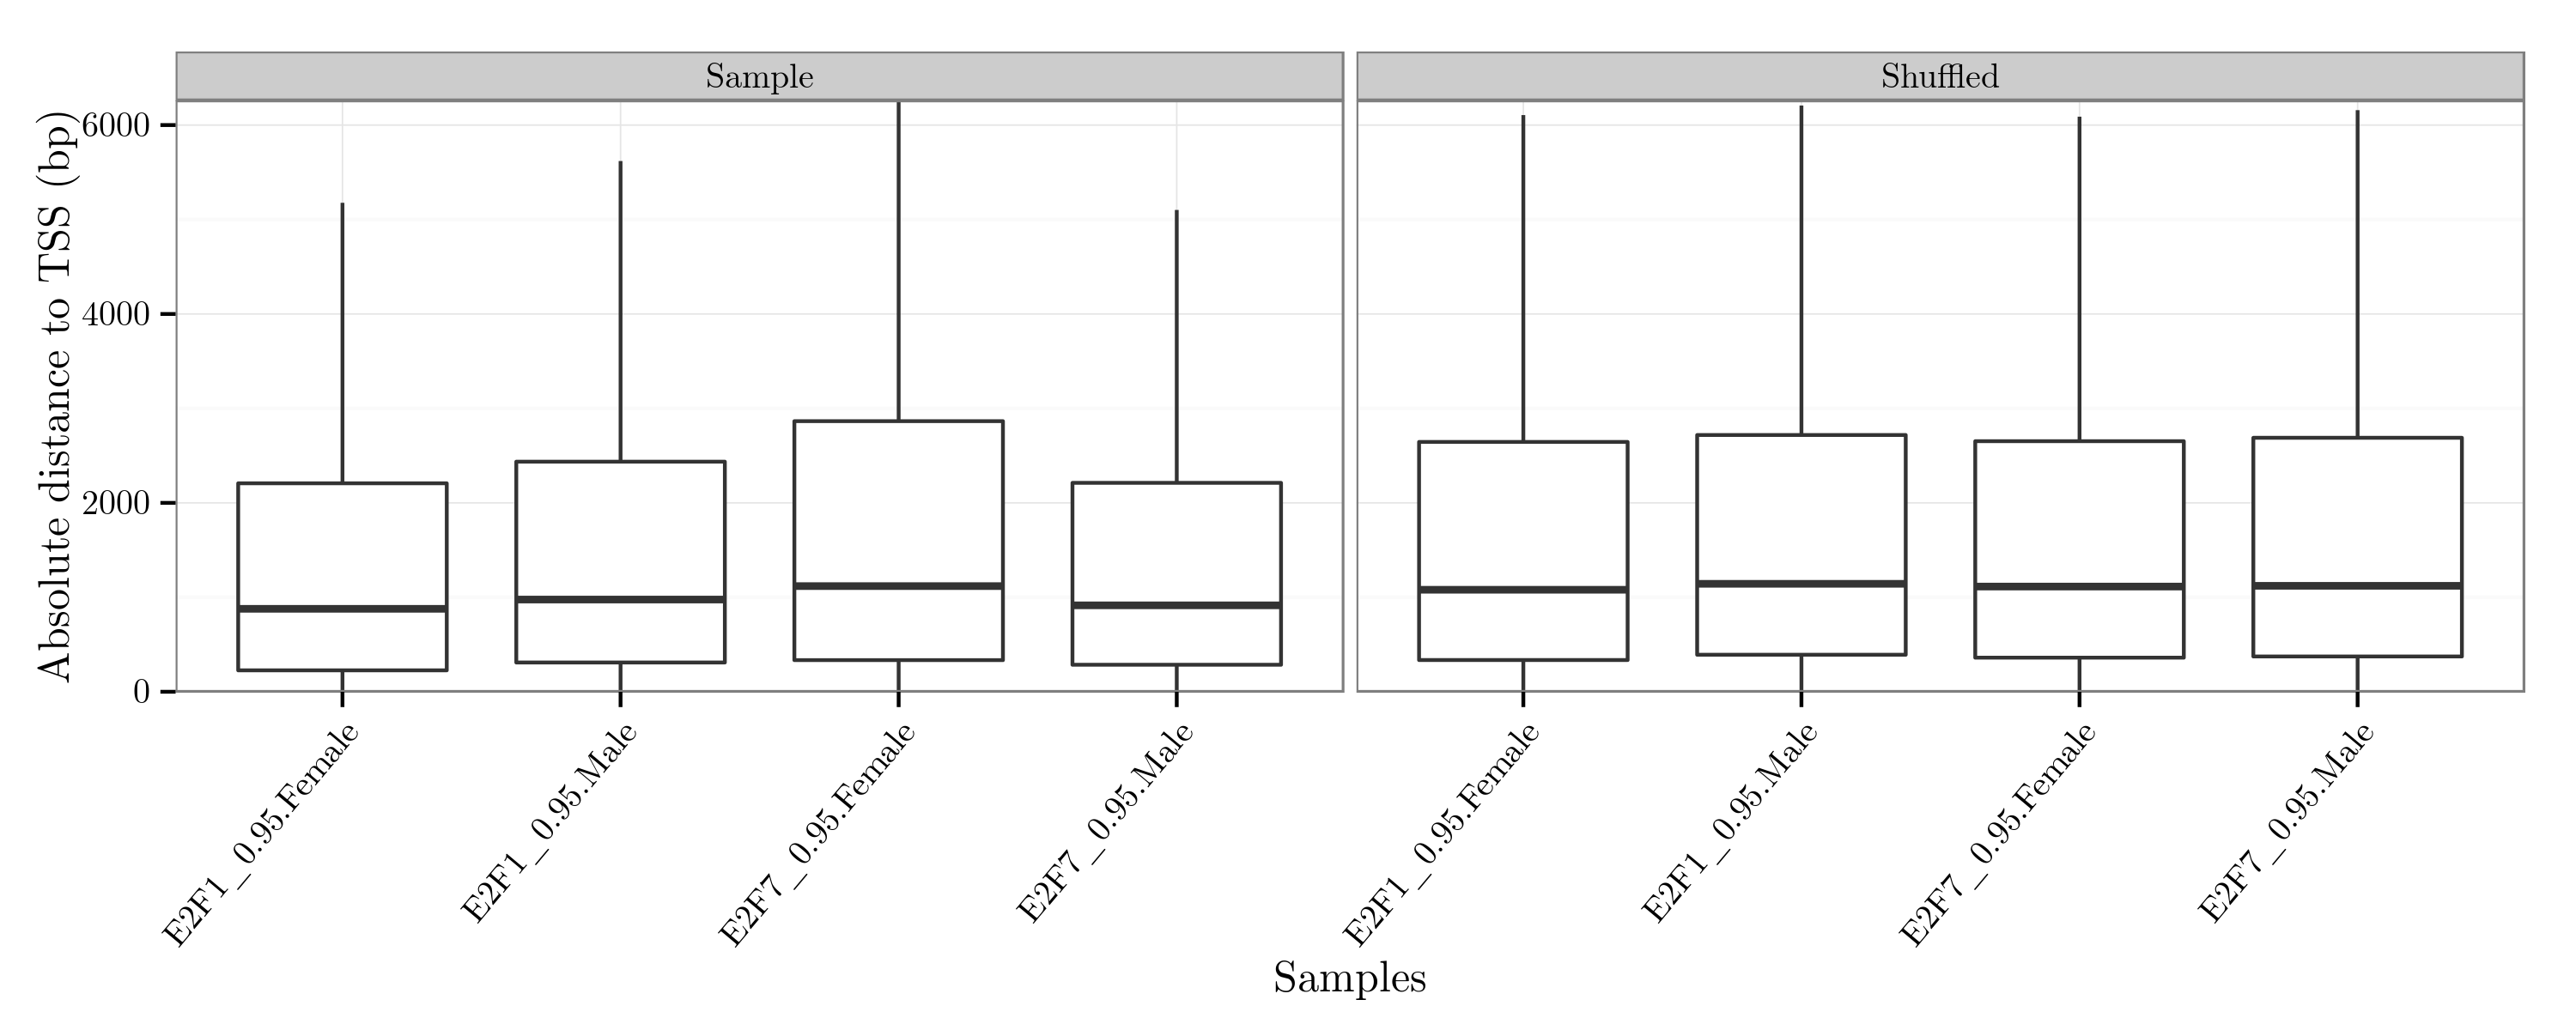
\includegraphics[width=1\linewidth]{pngs/E2F_distanceTSS_abs.png}
				\caption{Absolute distance.}
			\end{subfigure}
			\begin{subfigure}[b]{0.75\textwidth}
				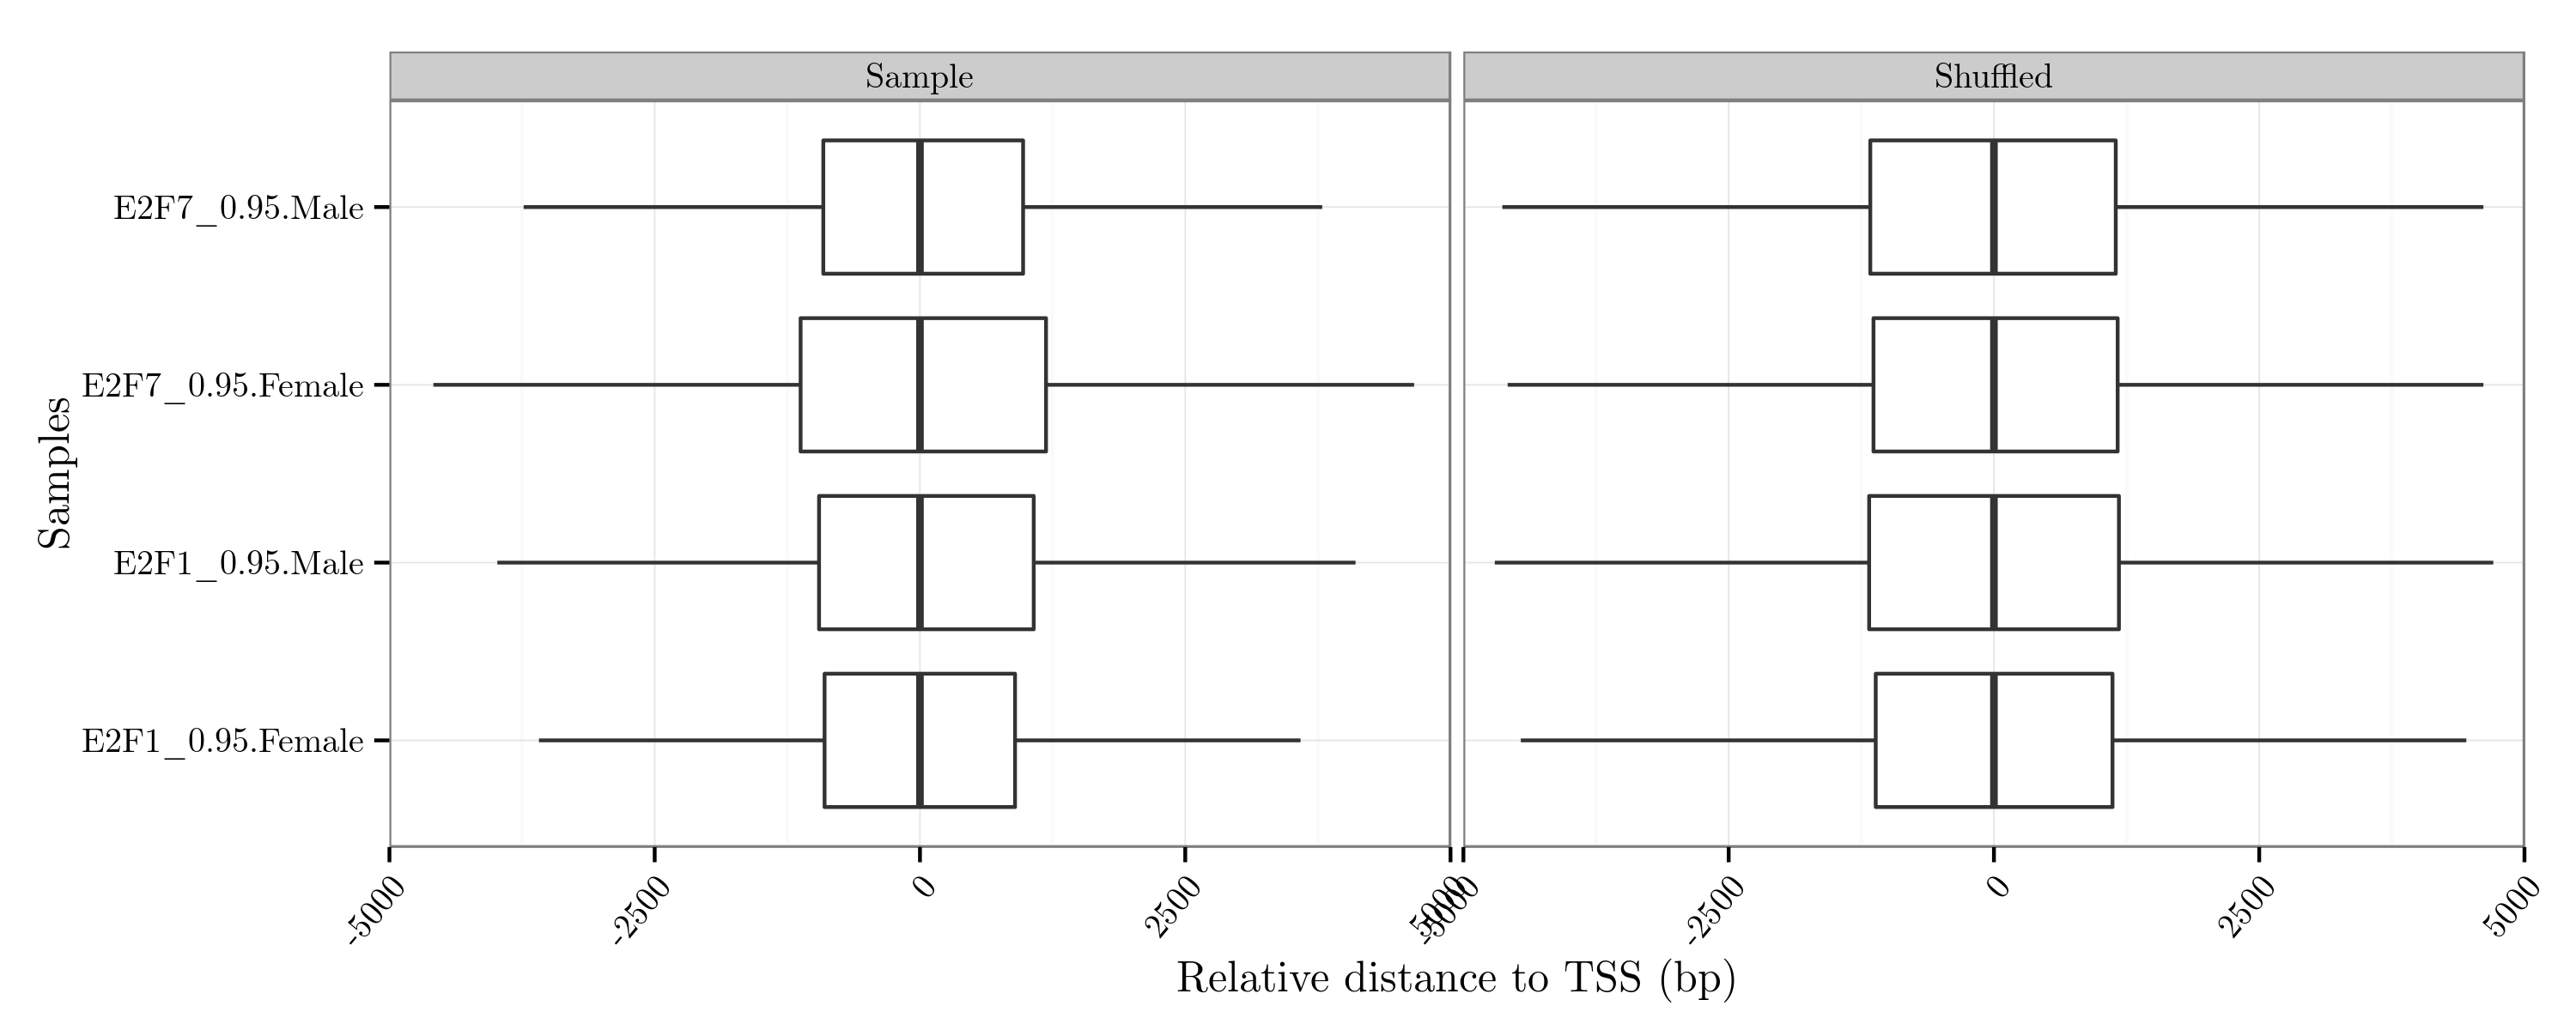
\includegraphics[width=1\linewidth]{pngs/E2F_distanceTSS_rel.png}
				\caption{Distance relative to the transcription start site.}
			\end{subfigure}
			\caption{Distance of E2F ChIP-ER to the nearest gene transcription start site.}\label{dummy}
			\label{fig:distance_to_TSS}
		\end{figure}
		
		E2F ChIP-ER are constrained by the genomic architecture and their genomic distribution resembles the background of the genome (Figure \ref{fig:genomic_location}).
		  		
		\begin{figure}[here]
			\centering
			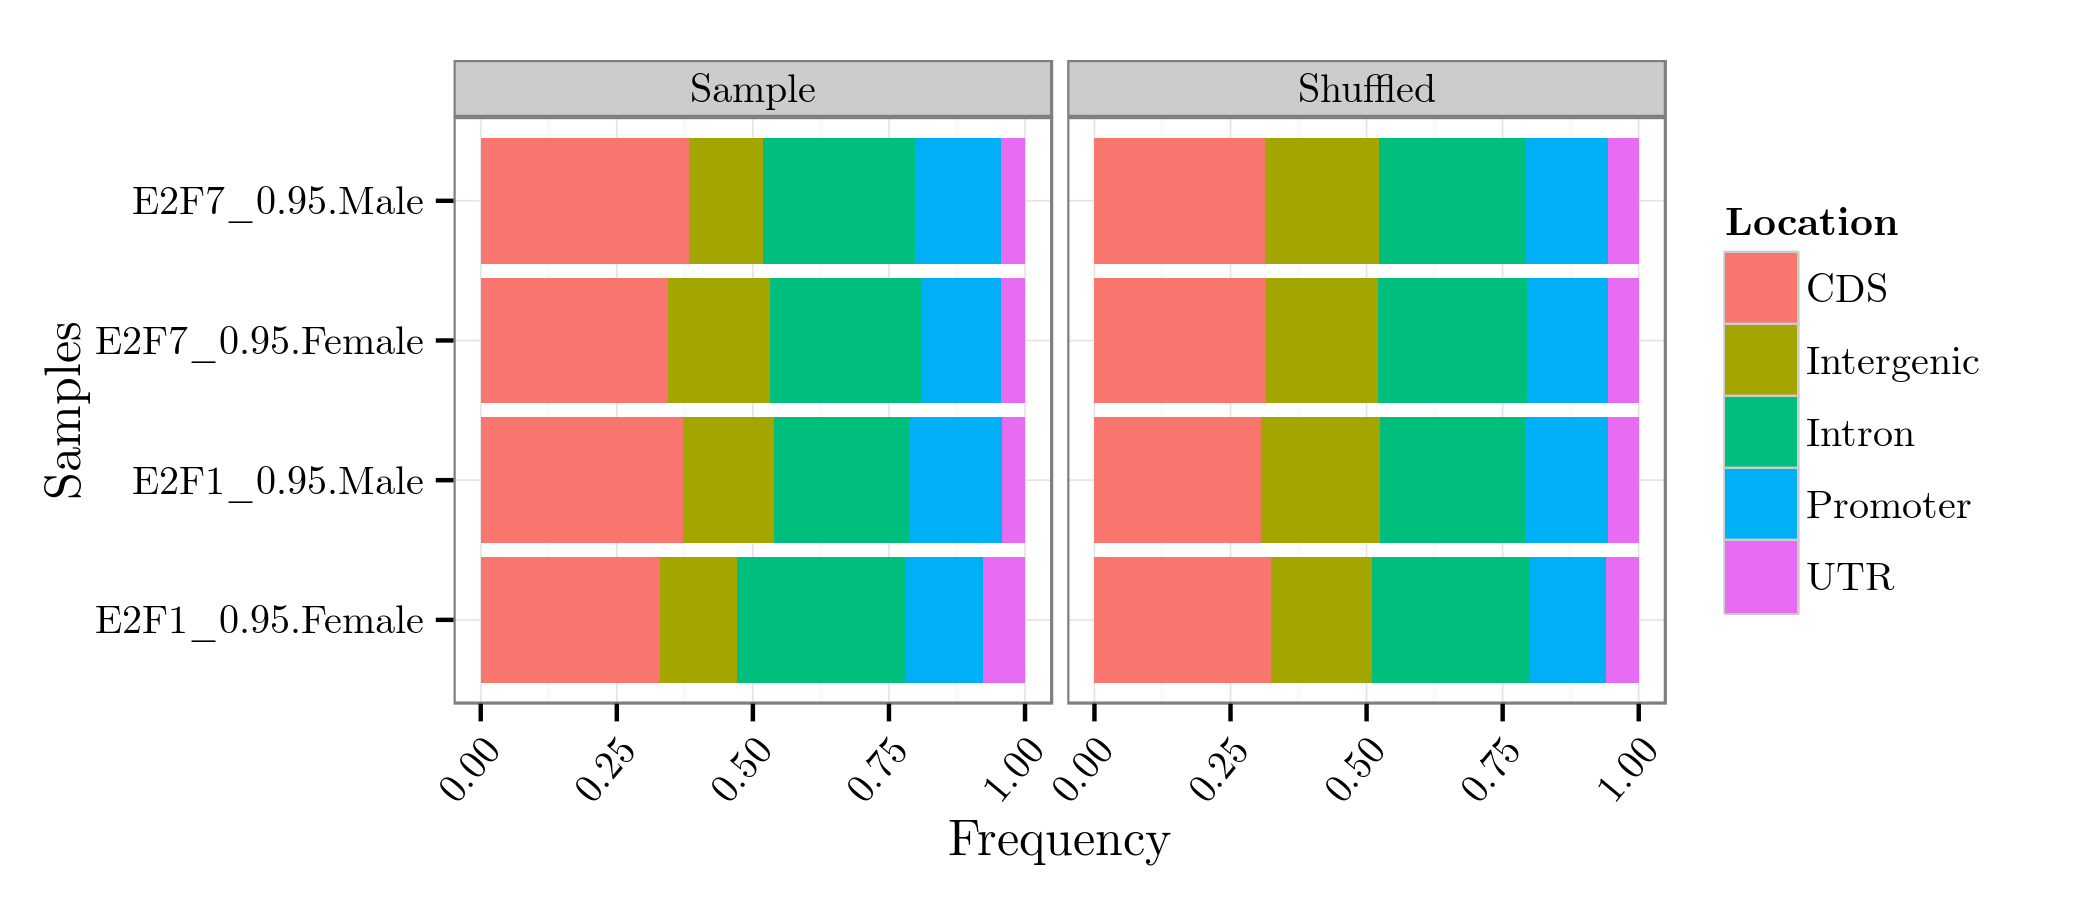
\includegraphics[width=0.9\textwidth]{pngs/E2F_genomicLocation.png}
			\caption{Location of E2F ChIP-ERs and shuffled regions of same number and width in the genome of \textit{Oikopleura dioica}.}
			\label{fig:genomic_location}
		\end{figure}
		
		E2F motifs found (Figure \ref{fig:E2F_motifs}).
		
		\begin{figure}[here]
			\centering
			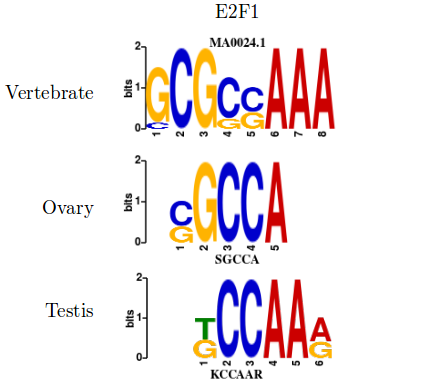
\includegraphics[width=0.5\textwidth]{pngs/E2F_motifs.png}
			\caption{Significant motifs found in E2F ChIP-ER that align with the known vertebrate E2F motif.}
			\label{fig:E2F_motifs}
		\end{figure}
		
		E2F ChIP-ER didn't show any particular correlations with the epigenetic landscape (Fig \ref{fig:E2F_Chromatin states}.
		
		\begin{figure}
			\setlength{\belowcaptionskip}{5pt}
			\centering
			\begin{subfigure}[b]{1\textwidth}
				\centering
				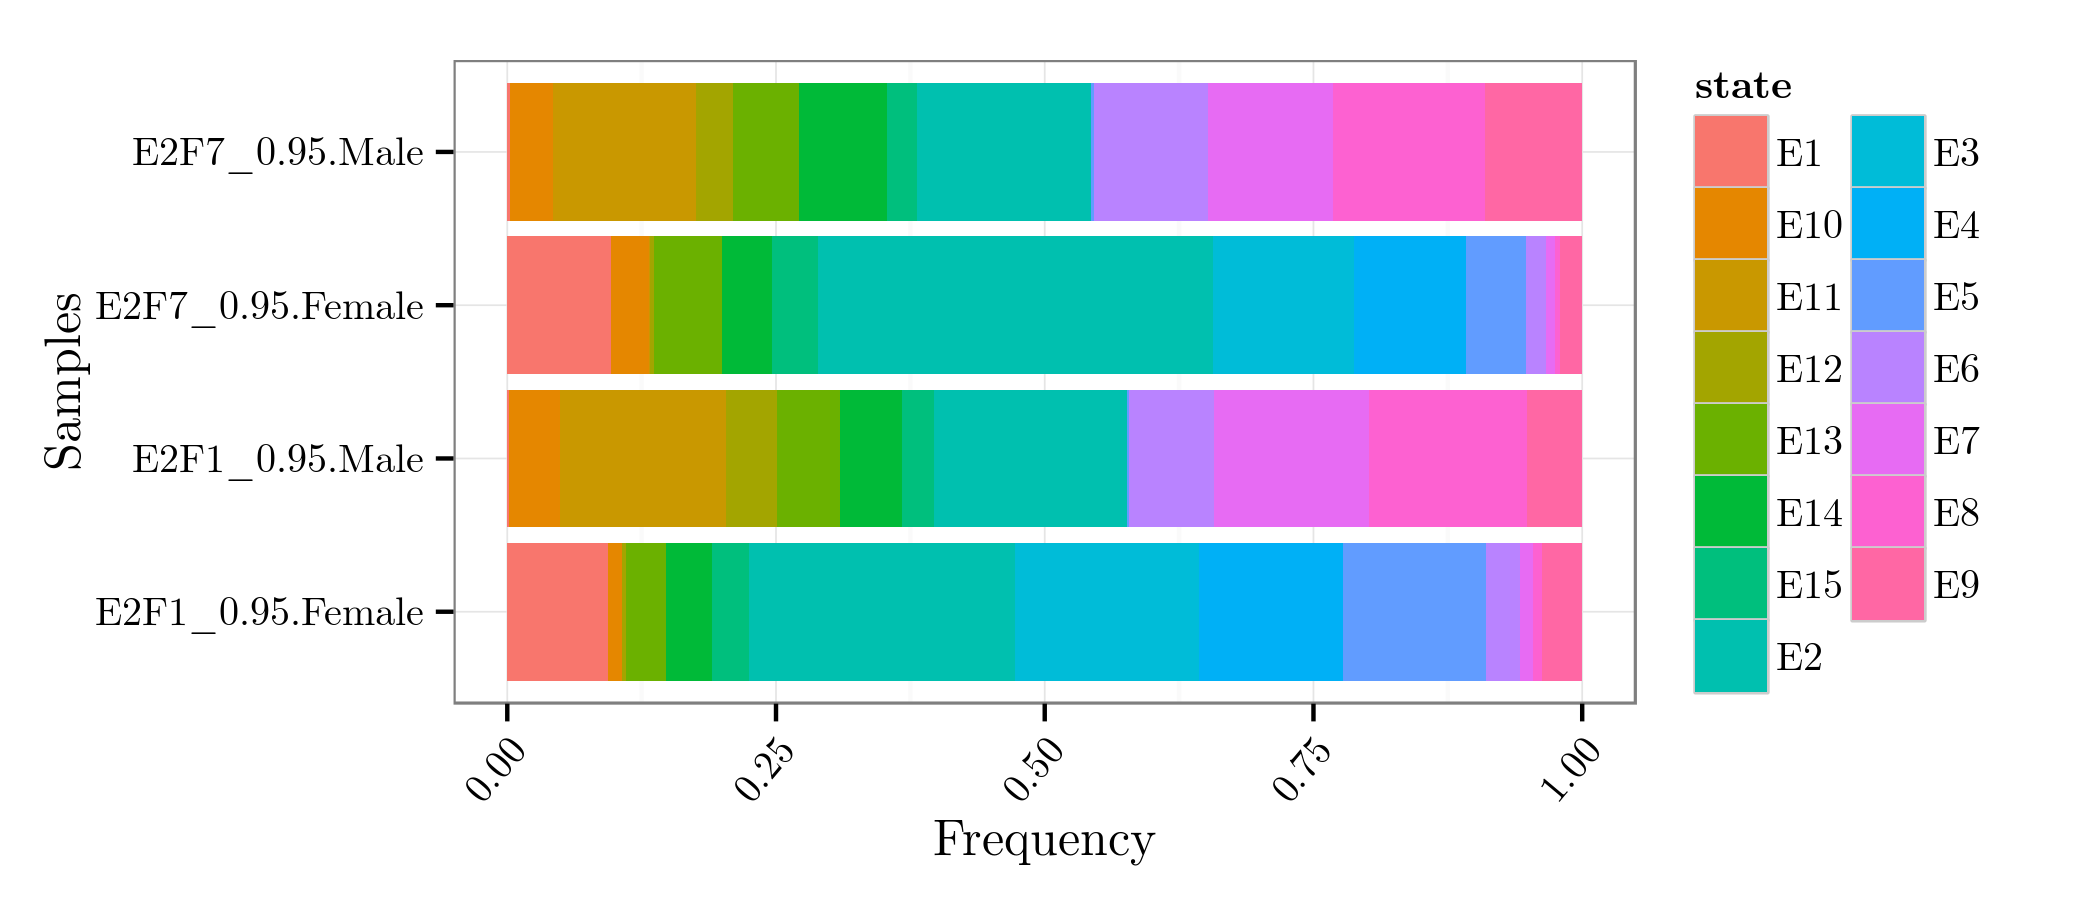
\includegraphics[width=1\linewidth]{pngs/E2F_chromatinAnnotation.png}
				\caption{Frequency of location of ChIP-ERs in the chromatin state annotation.}
			\end{subfigure}
			\begin{subfigure}[b]{1\textwidth}
				\centering
				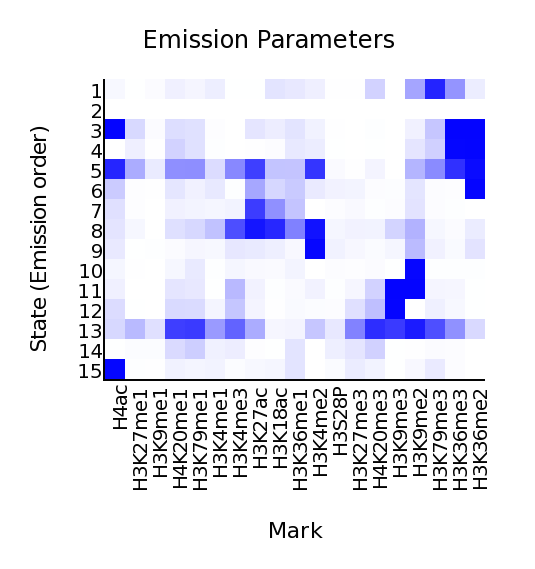
\includegraphics[width=0.5\linewidth]{pngs/ChromHMM_emissions_15.png}
				\caption{Composition of chromatin states based on histone modifications in \textit{Oikopleura dioica}.}
			\end{subfigure}
			\caption{Location of ChIP-enriched regions (CHIP-ER) regarding the local chromatin environment.
				{\footnotesize
				}
			}
			\label{fig:E2F_Chromatin_states}
		\end{figure}
		
		
    	E2F ChIP-ER showed high spatial and temporal co-localization within and between developmental stages (Figure \ref{fig:E2F_colocalization}).
    	
		\begin{figure}[here]
			\setlength{\belowcaptionskip}{5pt}
			\centering
			\begin{subfigure}[b]{0.75\textwidth}
				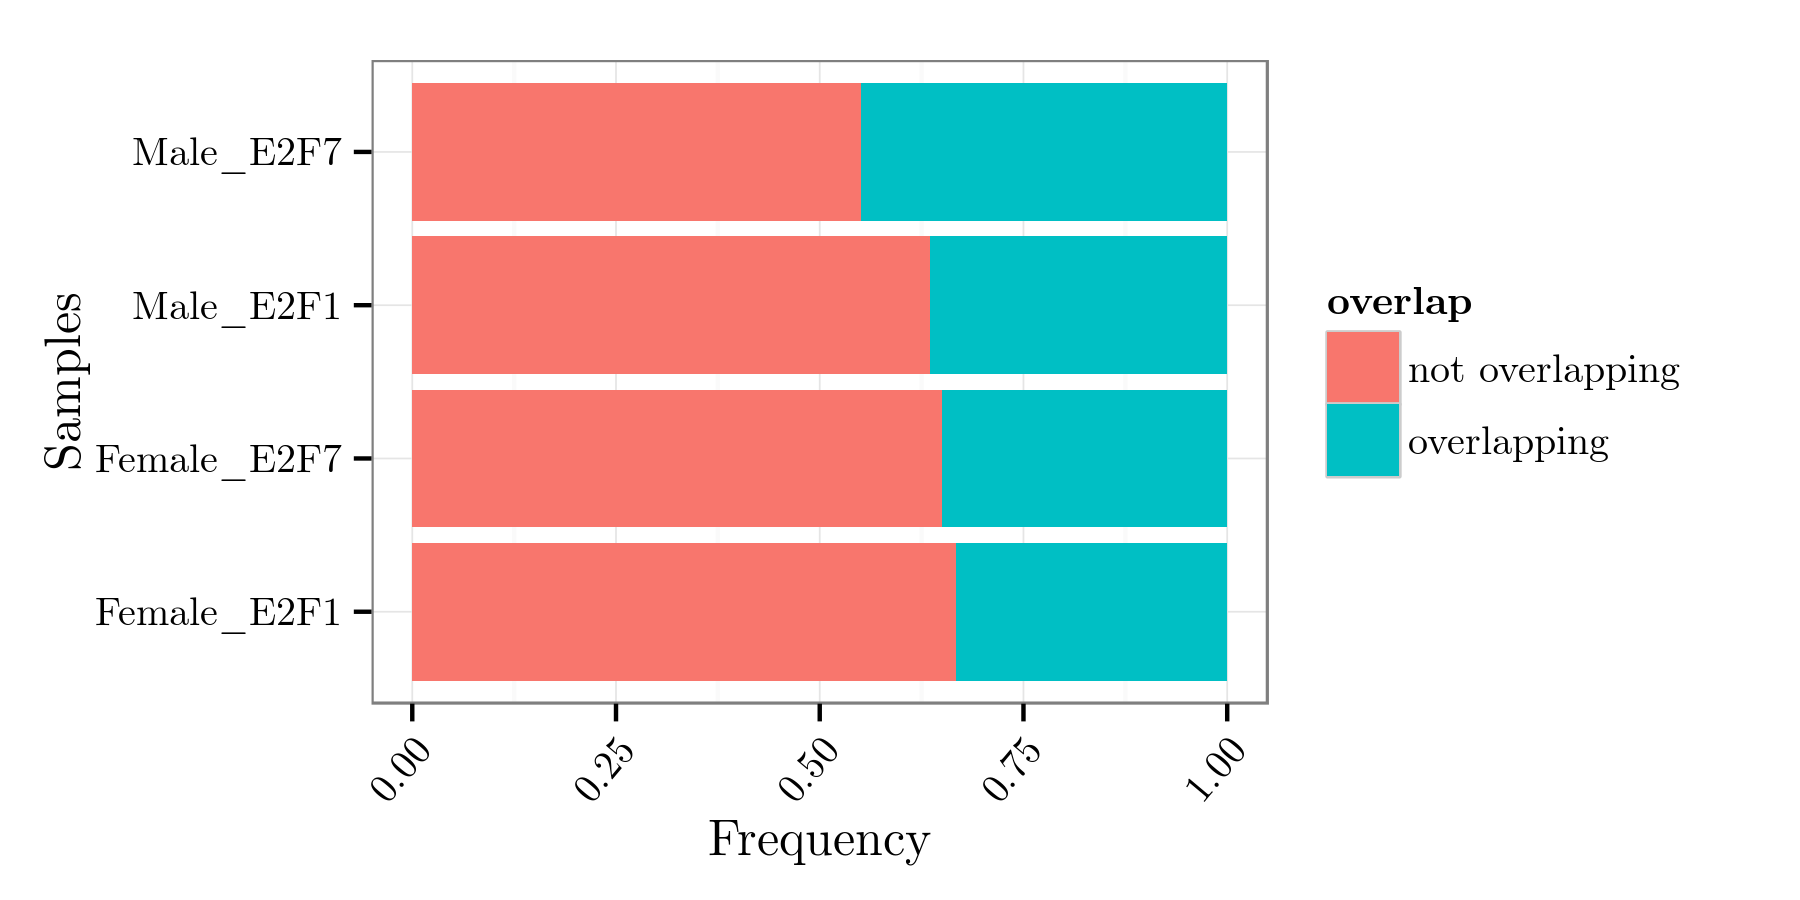
\includegraphics[width=1\linewidth]{pngs/E2F_overlap.png}
				\caption{Portion of ChIP-ERs that are shared (overlap) between transcription factors within the same developmental stage.}
			\end{subfigure}
			\begin{subfigure}[b]{0.75\textwidth}
				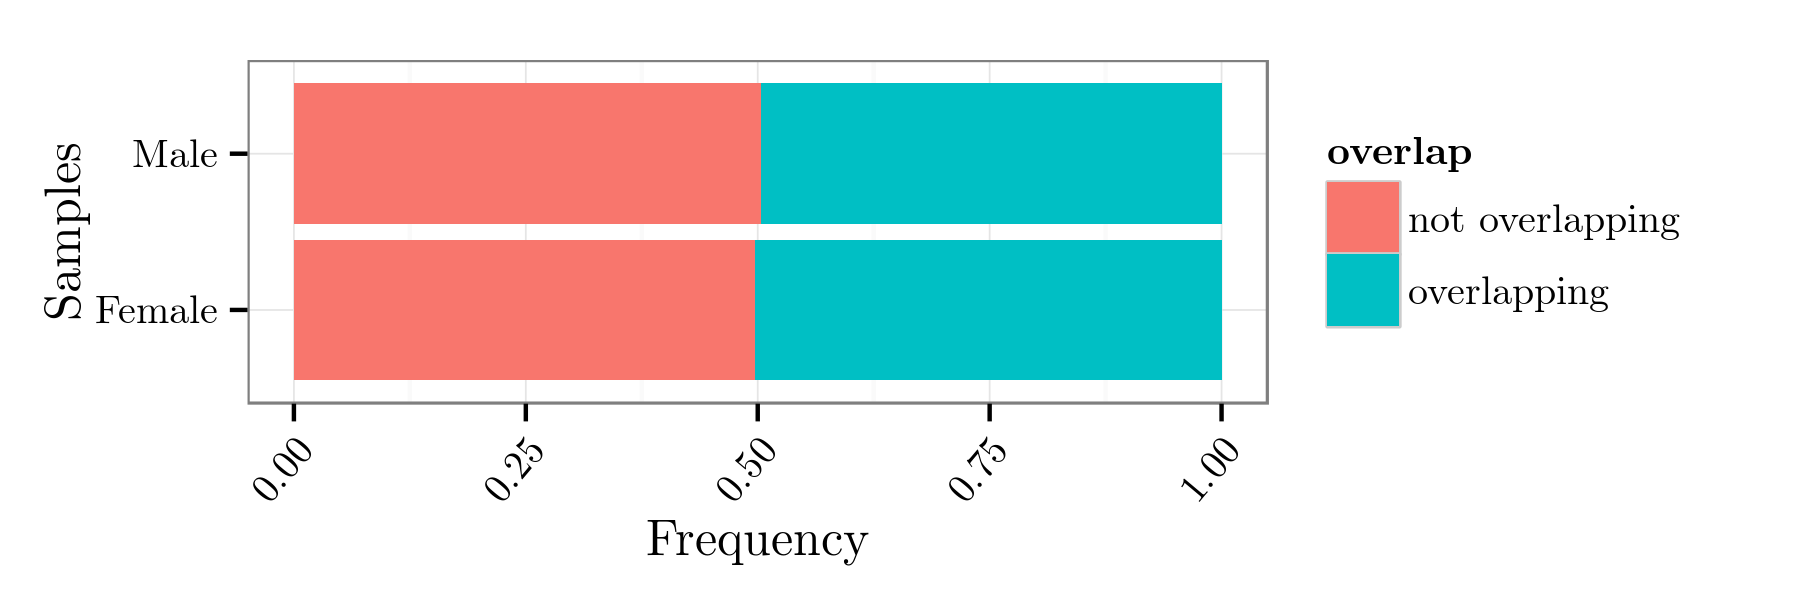
\includegraphics[width=1\linewidth]{pngs/E2F_overlap_overlaps.png}
				\caption{Portion of shared (overlapping) ChIP-ERs between transcription factors that also overlap between developmental stages.}
			\end{subfigure}
			\caption{Portion of E2F ChIP-ERs shared (overlapping) within and between developmental stages.}
			\label{fig:E2F_colocalization}
		\end{figure}
		
	\subsection{Putative E2F regulated genes}
		
    	E2F putatively regulated genes show significant enrichment of terms related with DNA replication, cell cycle regulation...,  (Figure \ref{fig:GO}).
		    	
		\begin{figure}[here]
			\centering
			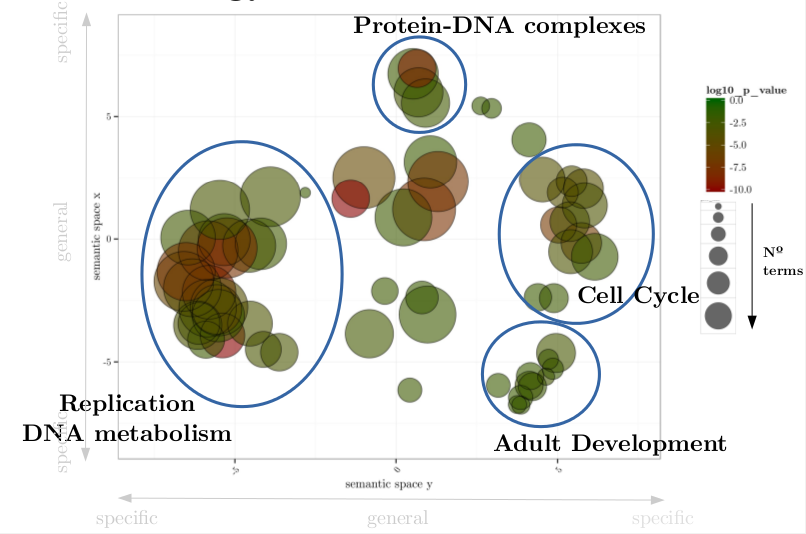
\includegraphics[width=0.9\textwidth]{pngs/E2F_overlap_overlaps_GO.png}
			\caption{Gene Ontology of genes putatively regulated by both E2F transcription factors in the D6 male developmental stage.
				{\footnotesize 
					Data spread over two semantic spaces (axis).
					Gene Ontology terms were nested within the same parent and the amount of terms clustered is shown by the area of the circle.
					Significance values are shown in a color spectra.
					D6 female developmental stage have a high degree of similarity.
				}
			}
			\label{fig:GO}
		\end{figure}

    	There are major and significant changes at the transcriptome level between the D6 female and male developmental stages (Figure \ref{fig:D6_expression}).
		
		\begin{figure}[here]
			\centering
			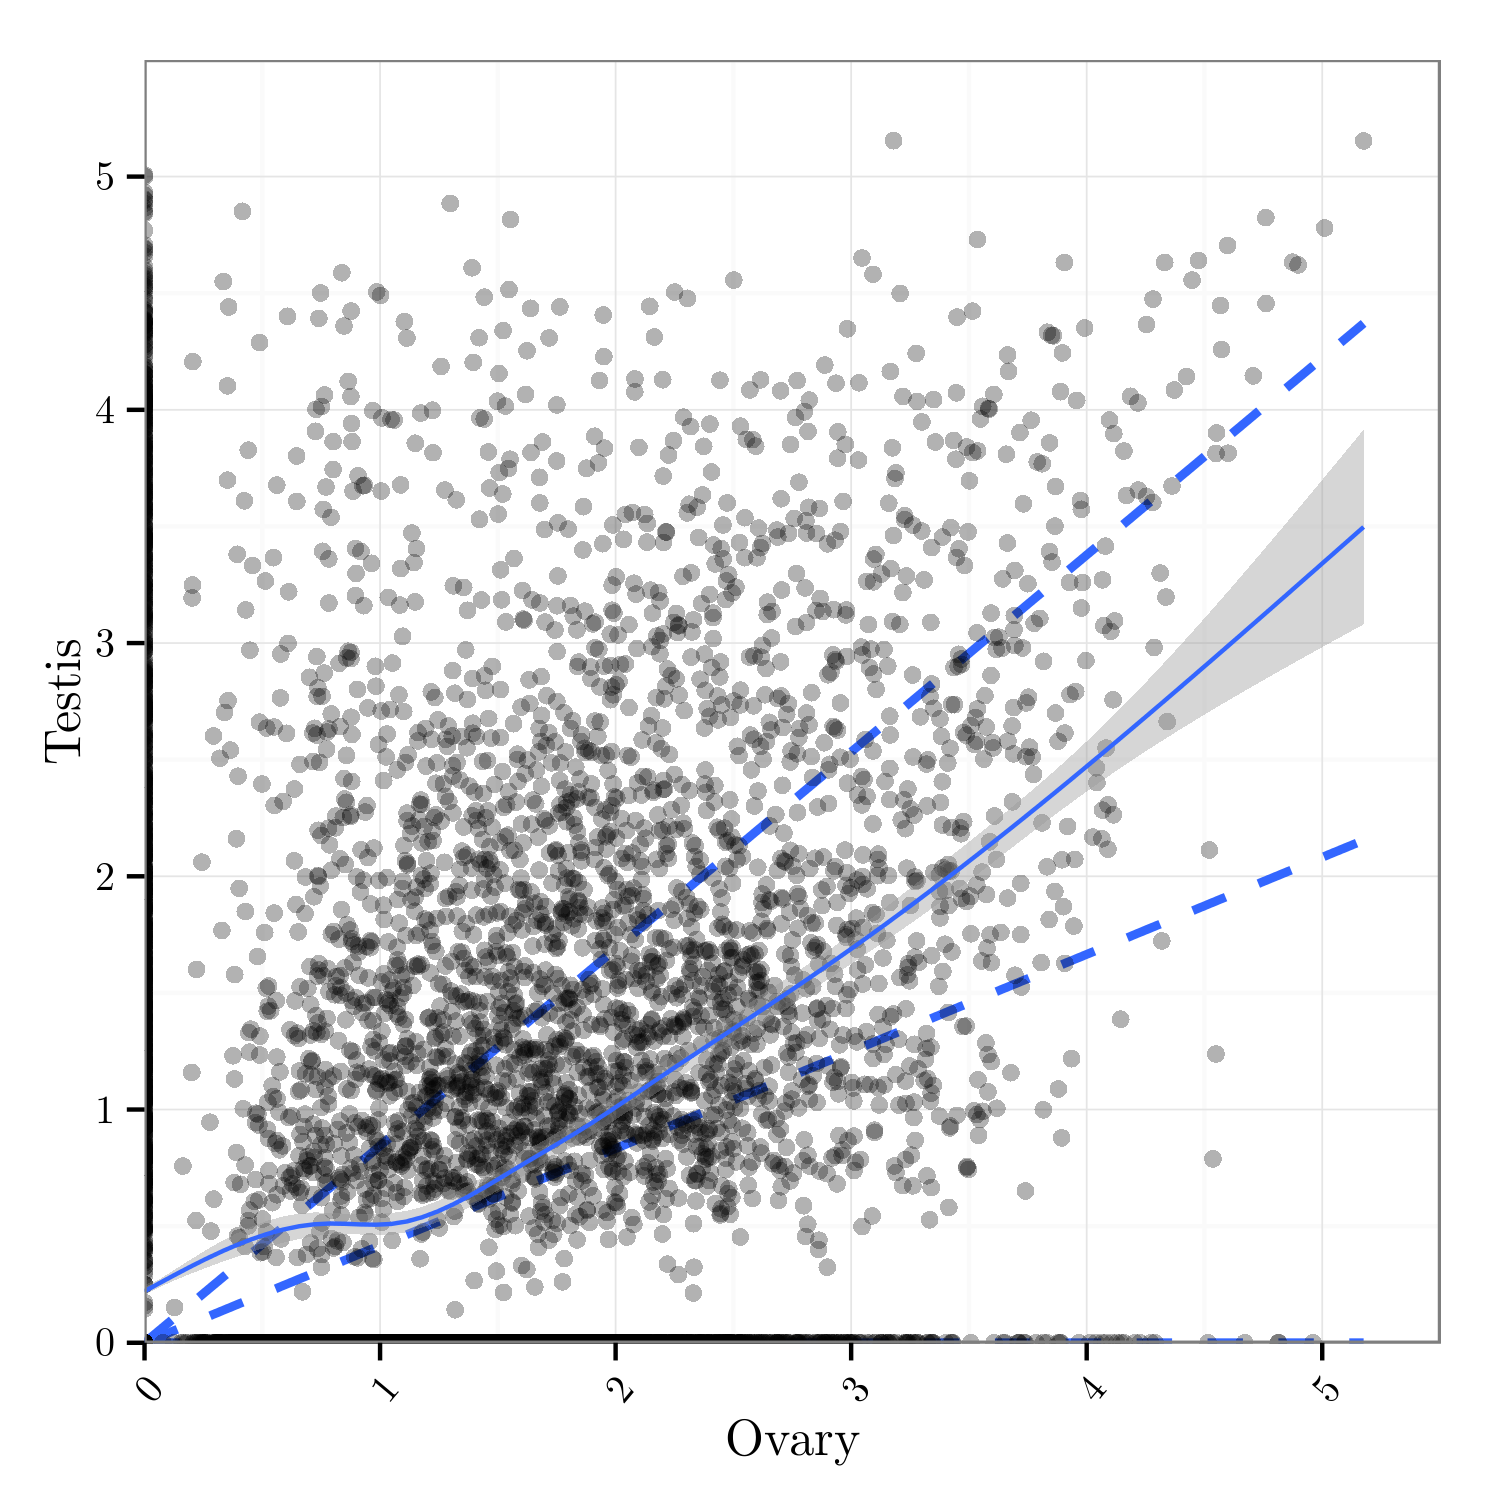
\includegraphics[width=0.5\textwidth]{pngs/D6_expression.png}
			\caption{Expression values of all genes in the D6 male (Testis) and D6 female (Ovary) developmental stages.
			{\footnotesize
				Expression values were normalized by the mean expression of all genes within each stage and transformed with a logarithm of base 2;
				Dashed lines indicate quantiles of the distribution of expression values;
				Smoothed line represents the smoothed conditional mean of expression values.
				}
			}
			\label{fig:D6_expression}
		\end{figure}

    	There were no significant changes between the means of the distribution of expression values of genes putatively regulated by E2F factors (Figure \ref{fig:E2F_targets_expression}).	However, a trend exists for genes that are bound by the repressor transcription factor (E2F7) in a stage to be less expressed in that stage and more in the other.
		
		\begin{figure}
			\centering
			\begin{subfigure}{.5\textwidth}
				\centering
				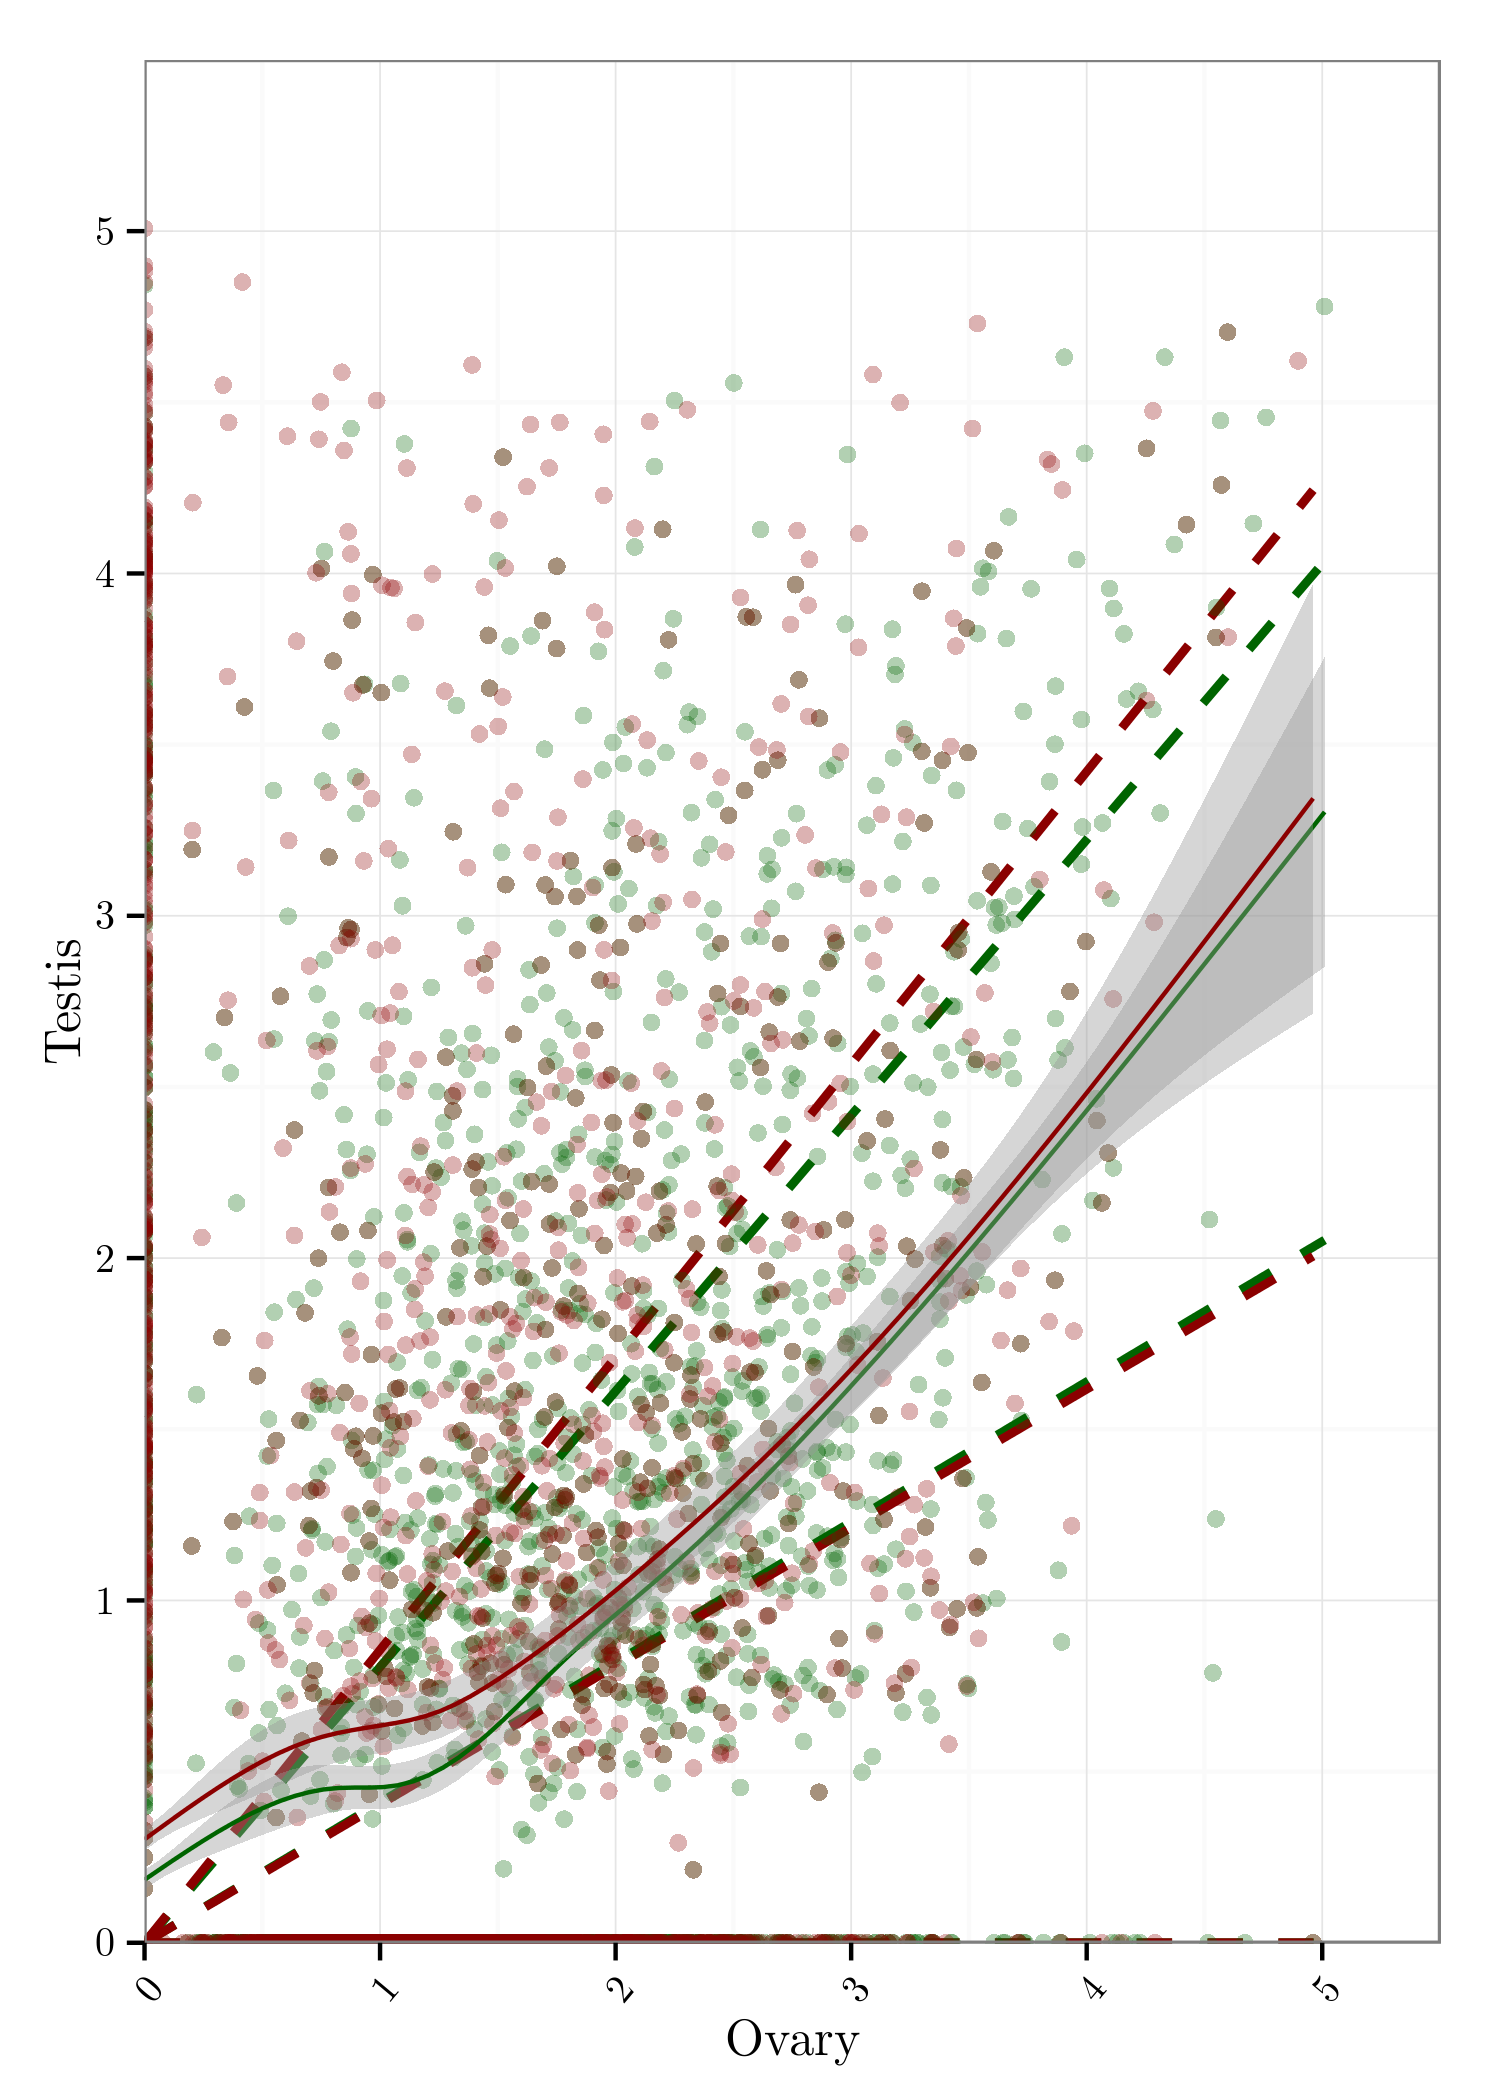
\includegraphics[width=1\linewidth]{pngs/E2F_specific_Female_expression.png}
				\caption{D6 Female developmental stage (Ovary).}
			\end{subfigure}%
			\begin{subfigure}{.5\textwidth}
				\centering
				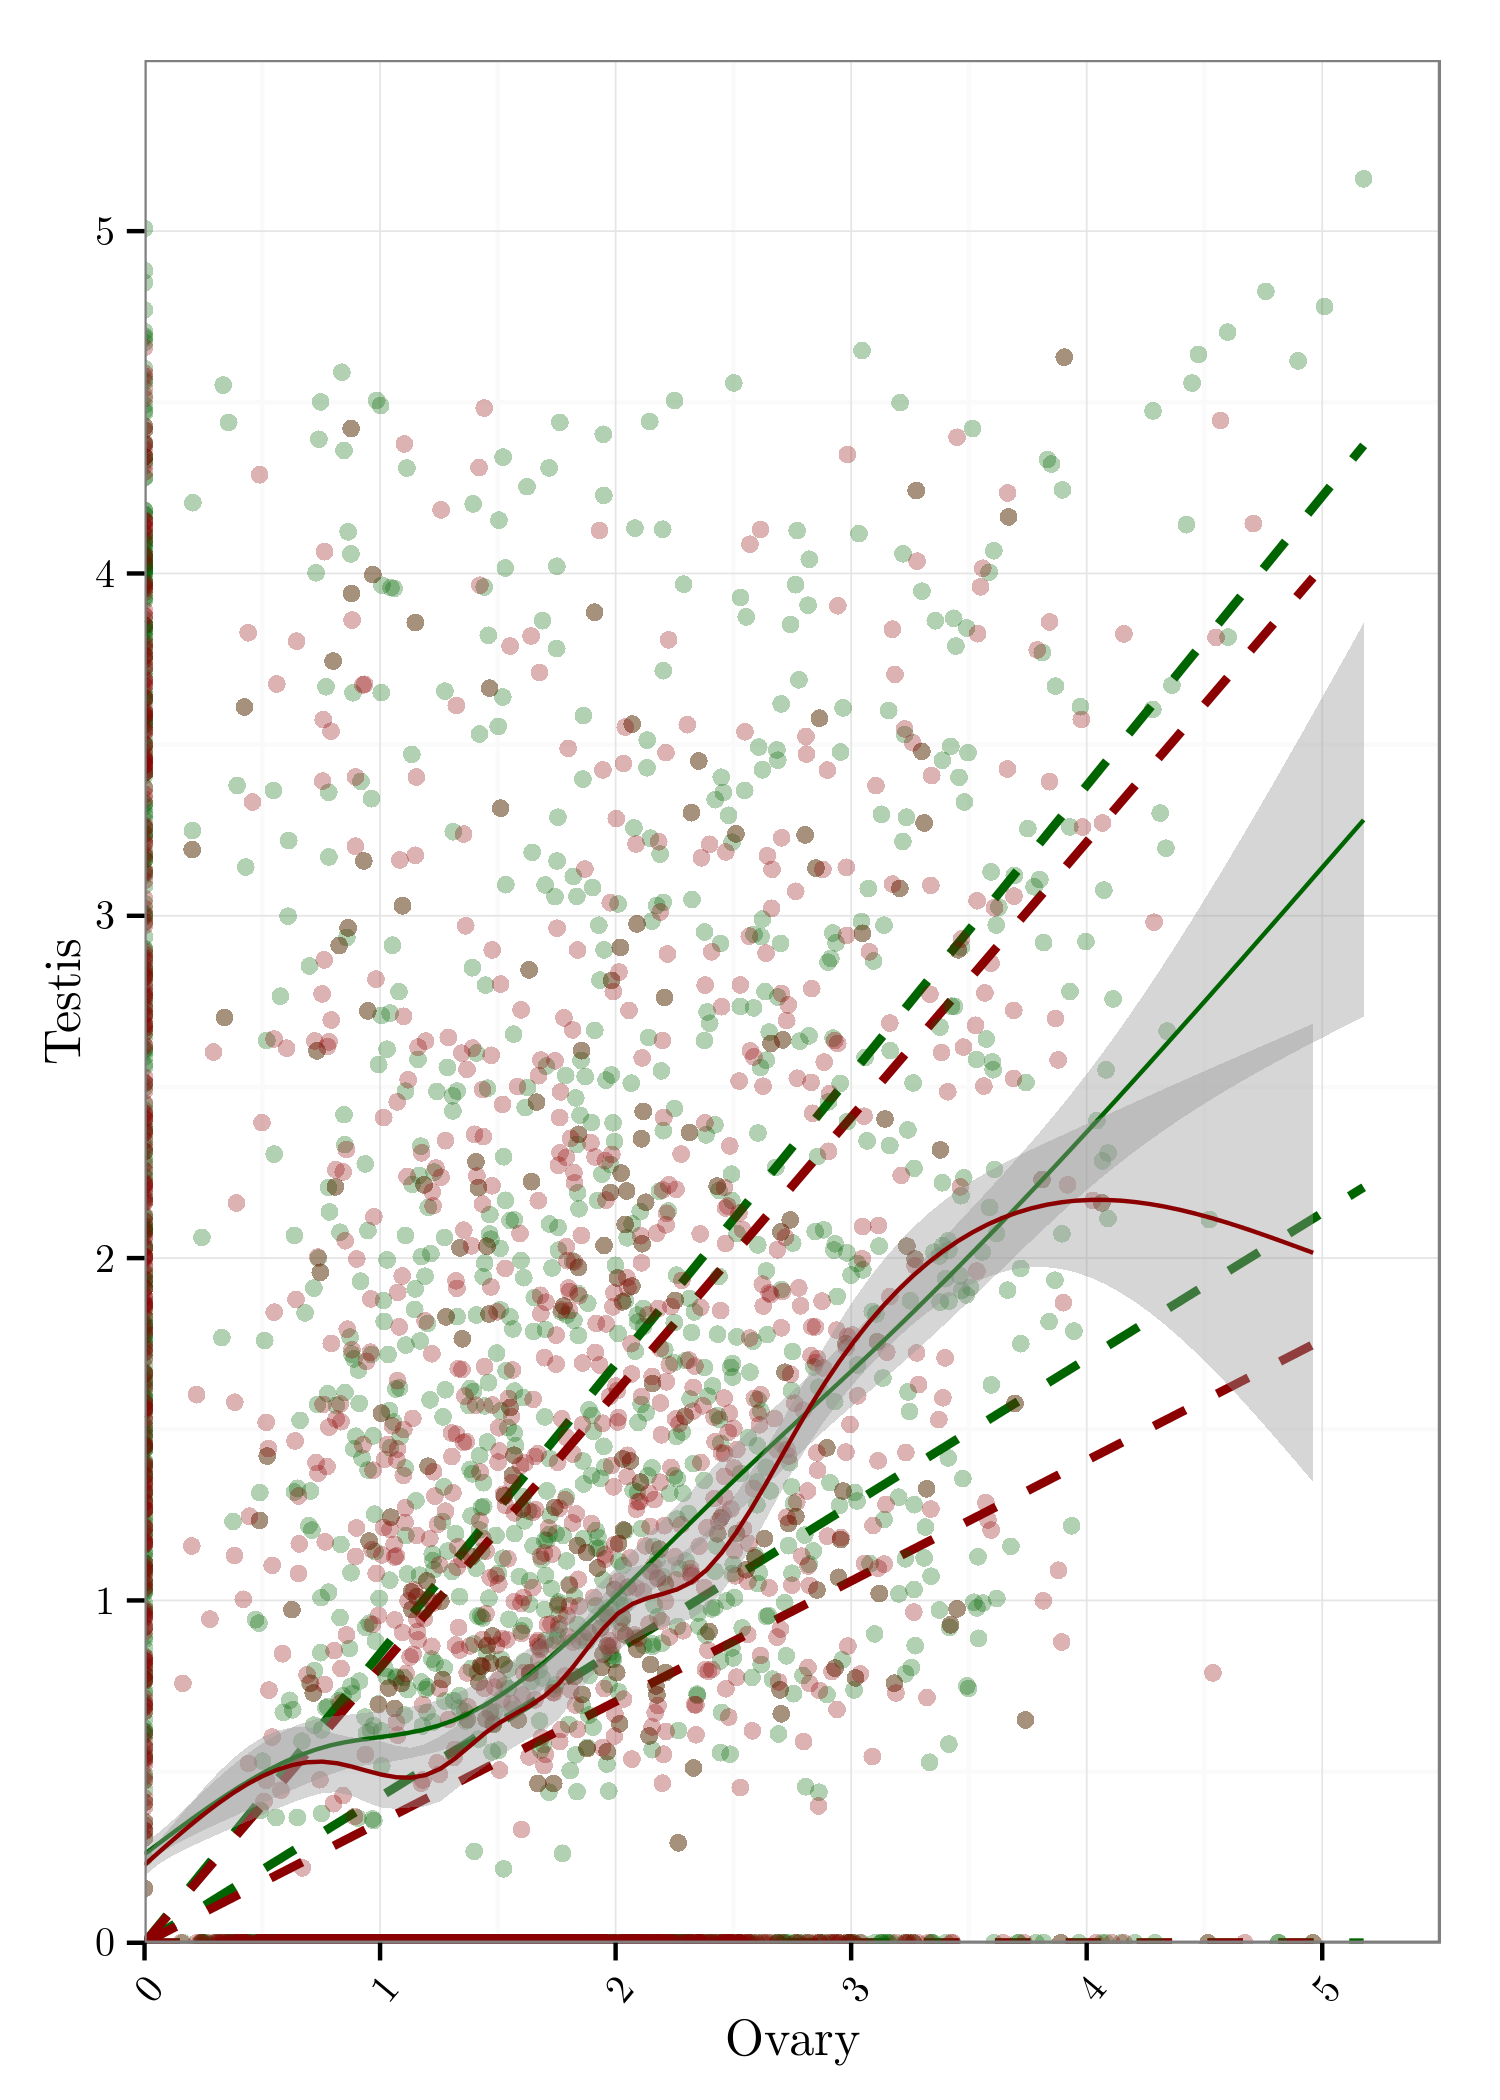
\includegraphics[width=1\linewidth]{pngs/E2F_specific_Male_expression.png}
				\caption{D6 Male developmental stage (Testis).}
			\end{subfigure}
			\caption{Expression values of genes putatively regulated by E2F transcription factors in the two developemtal stages where E2F binding was characterized.
			Green: E2F1-bound genes;
			Red: E2F7-bound genes;
				{\footnotesize
				Expression values were normalized by the mean expression of all genes within each stage and transformed with a logarithm of base 2;
				Dashed lines indicate quantiles of the distribution of expression values;
				Smoothed line represents the smoothed conditional mean of expression values.
				}
			}
			\label{fig:E2F_targets_expression}
		\end{figure}
		
		Key cell cycle regulators putatively regulated by E2F factors (see full list in appendix \ref{list_key_cell_cycle_regulators}).


\section{Dot1 and H3K79 methylation in \textit{Oikopleura dioica}'s cell cycle modes}
	
	Expression of Dot1 and Bre1 during \textit{Oikopleura dioica}'s development (Figure \ref{fig:Dot1_Bre1_expression}).
	
	\begin{figure}
		\centering
		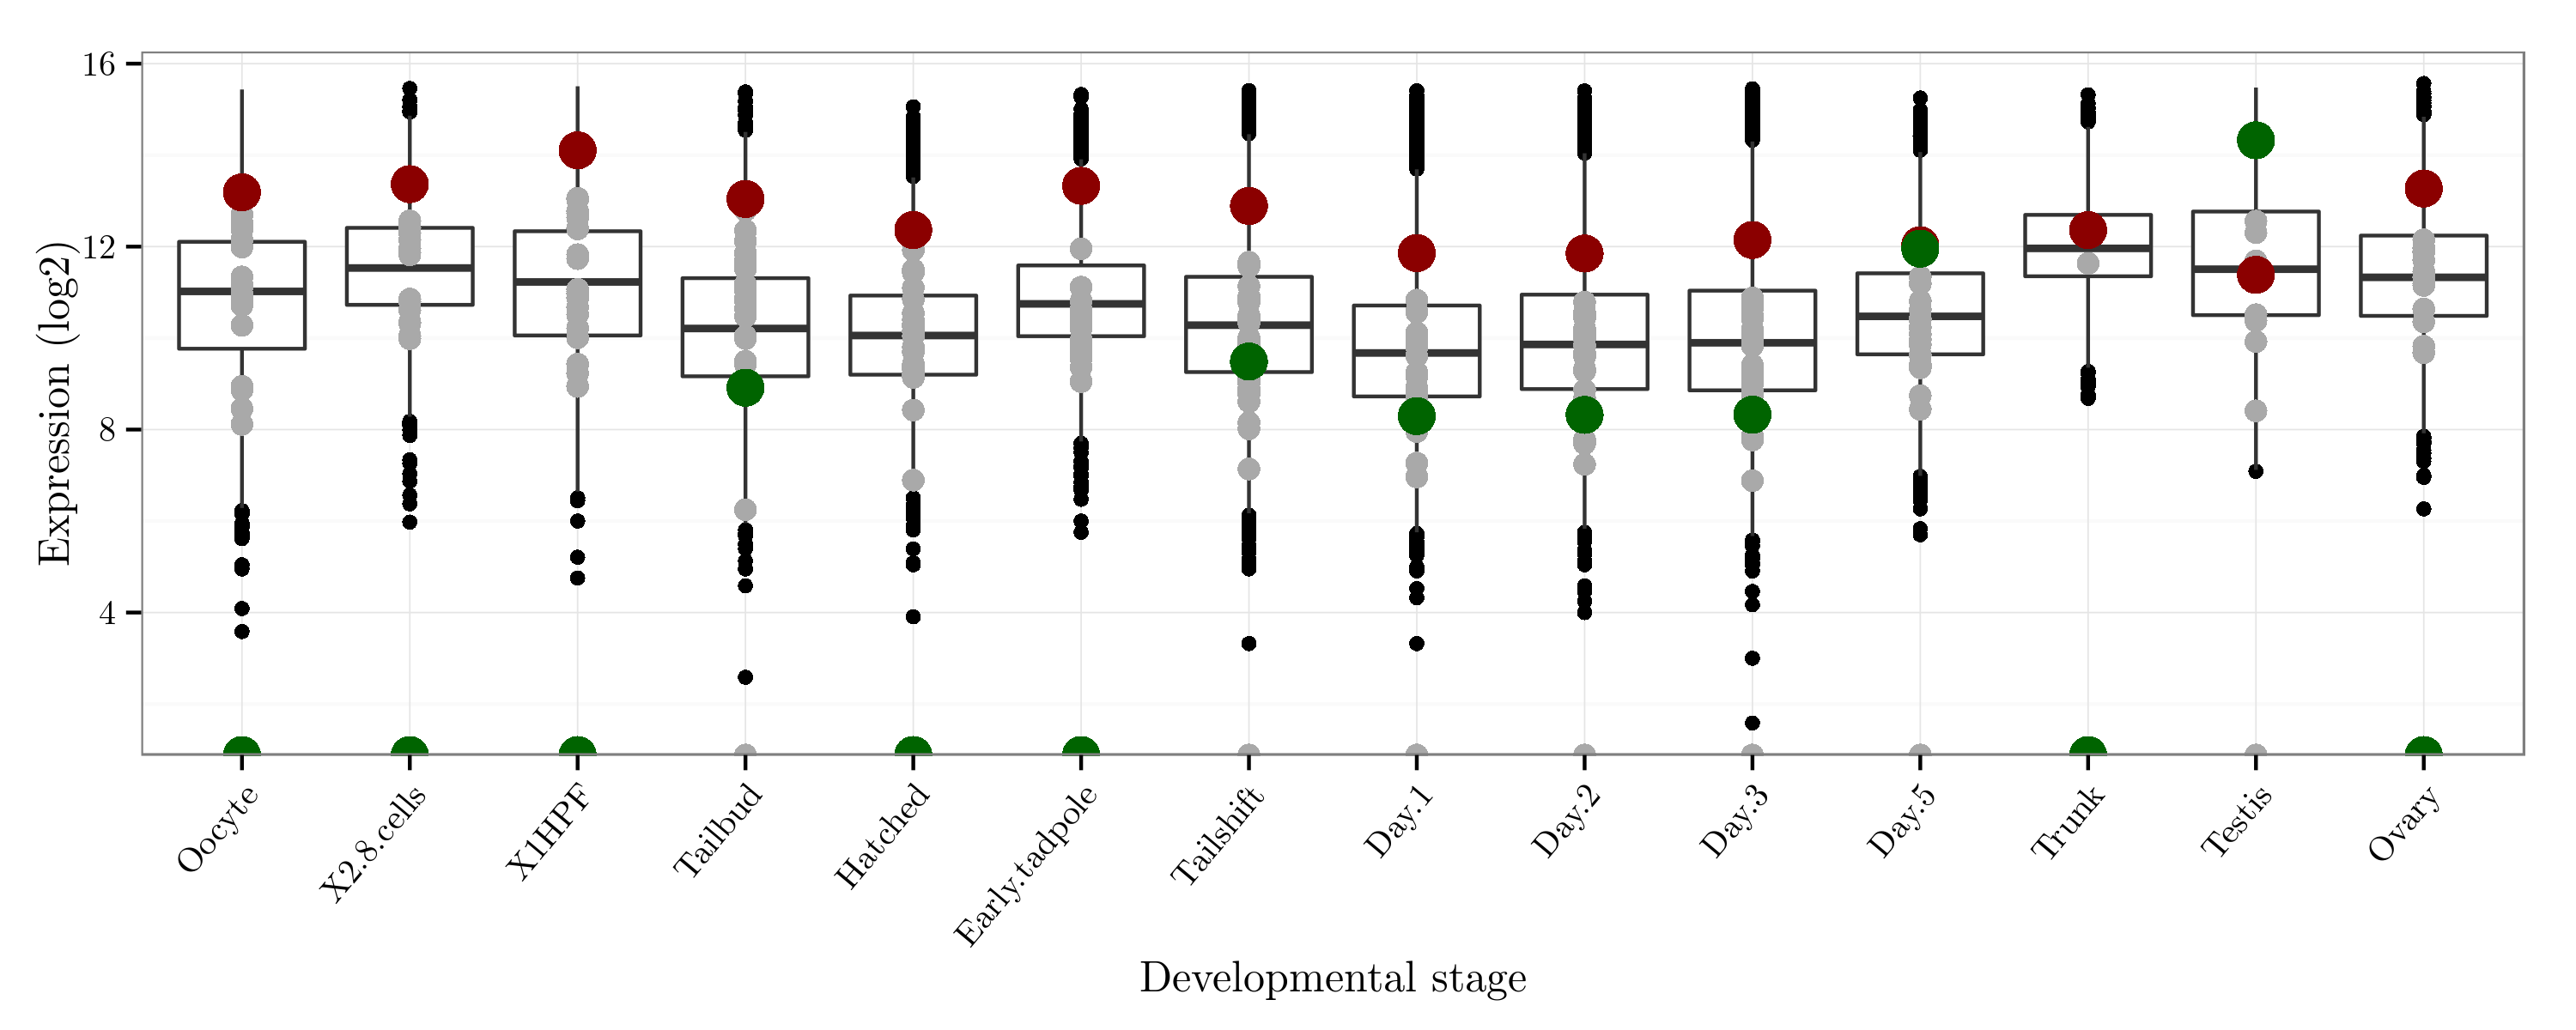
\includegraphics[width=1\textwidth]{pngs/Dot1_expression_allgenes_SETs.png}
		\caption{Expression values of Dot1 and Bre1 enzymes during (A) normal \textit{Oikopleura} development and growth arrest, and (B) after release from the growth arrest condition.
		Red: Bre1;
		Green: Dot1;
			{\footnotesize
			Expression values were transformed with a logarithm of base 2.
			}
		}
		\label{fig:Dot1_Bre1_expression}
	\end{figure}
	
	\textit{Oikopleura} is known to have a develop a condition with reduced proliferation and growth during dense culture due to reduced nutritional resources, known as growth arrest.  During growth arrest, expression of the Bre1 ubiquitin ligase is significantly reduced whereas the Dot1 methyltransferase is relatively stable (Figure \ref{fig:Dot1_Bre1_GA_expression}a). When animals are released from the growth arrest condition by restoring the normal culture density and nutritional supply, Bre1 expression is restored to levels compared with normal development during endocycling stages (Figure \ref{fig:Dot1_Bre1_GA_expression}b).	
	
	\begin{figure}
		\centering
		\begin{subfigure}{.5\textwidth}
			\centering
			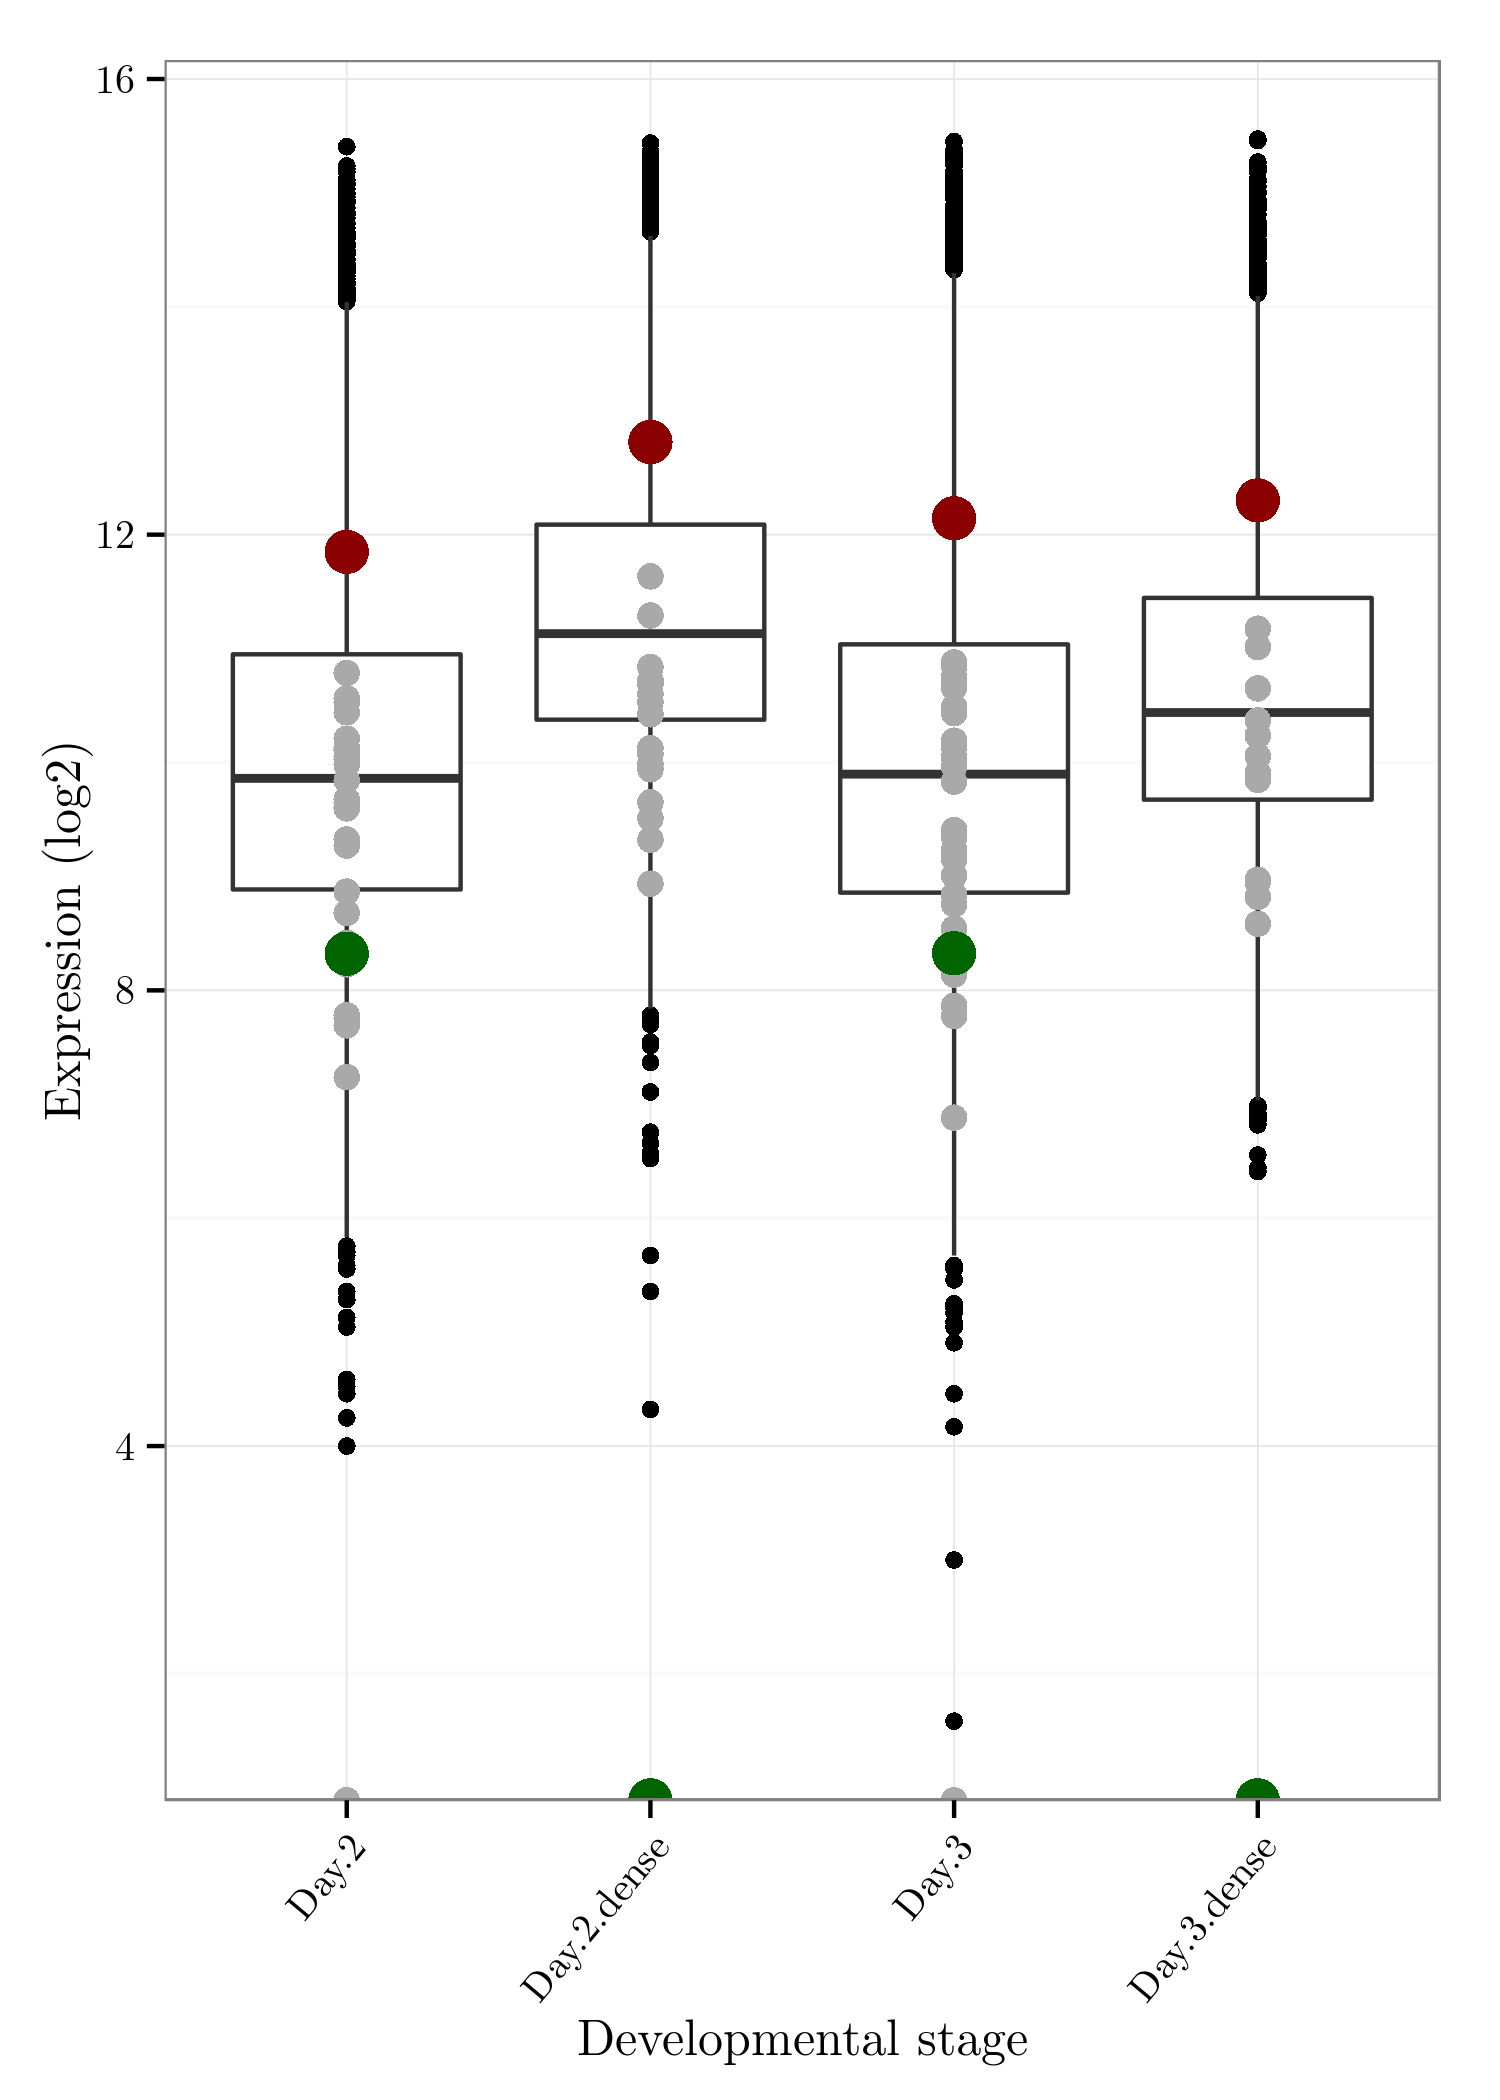
\includegraphics[width=1\linewidth]{pngs/Dot1_expression_allgenes_SETs_dense_noDay4.png}
			\caption{Expression during normal culture and growth arrest conditions.}
		\end{subfigure}%
		\begin{subfigure}{.5\textwidth}
			\centering
			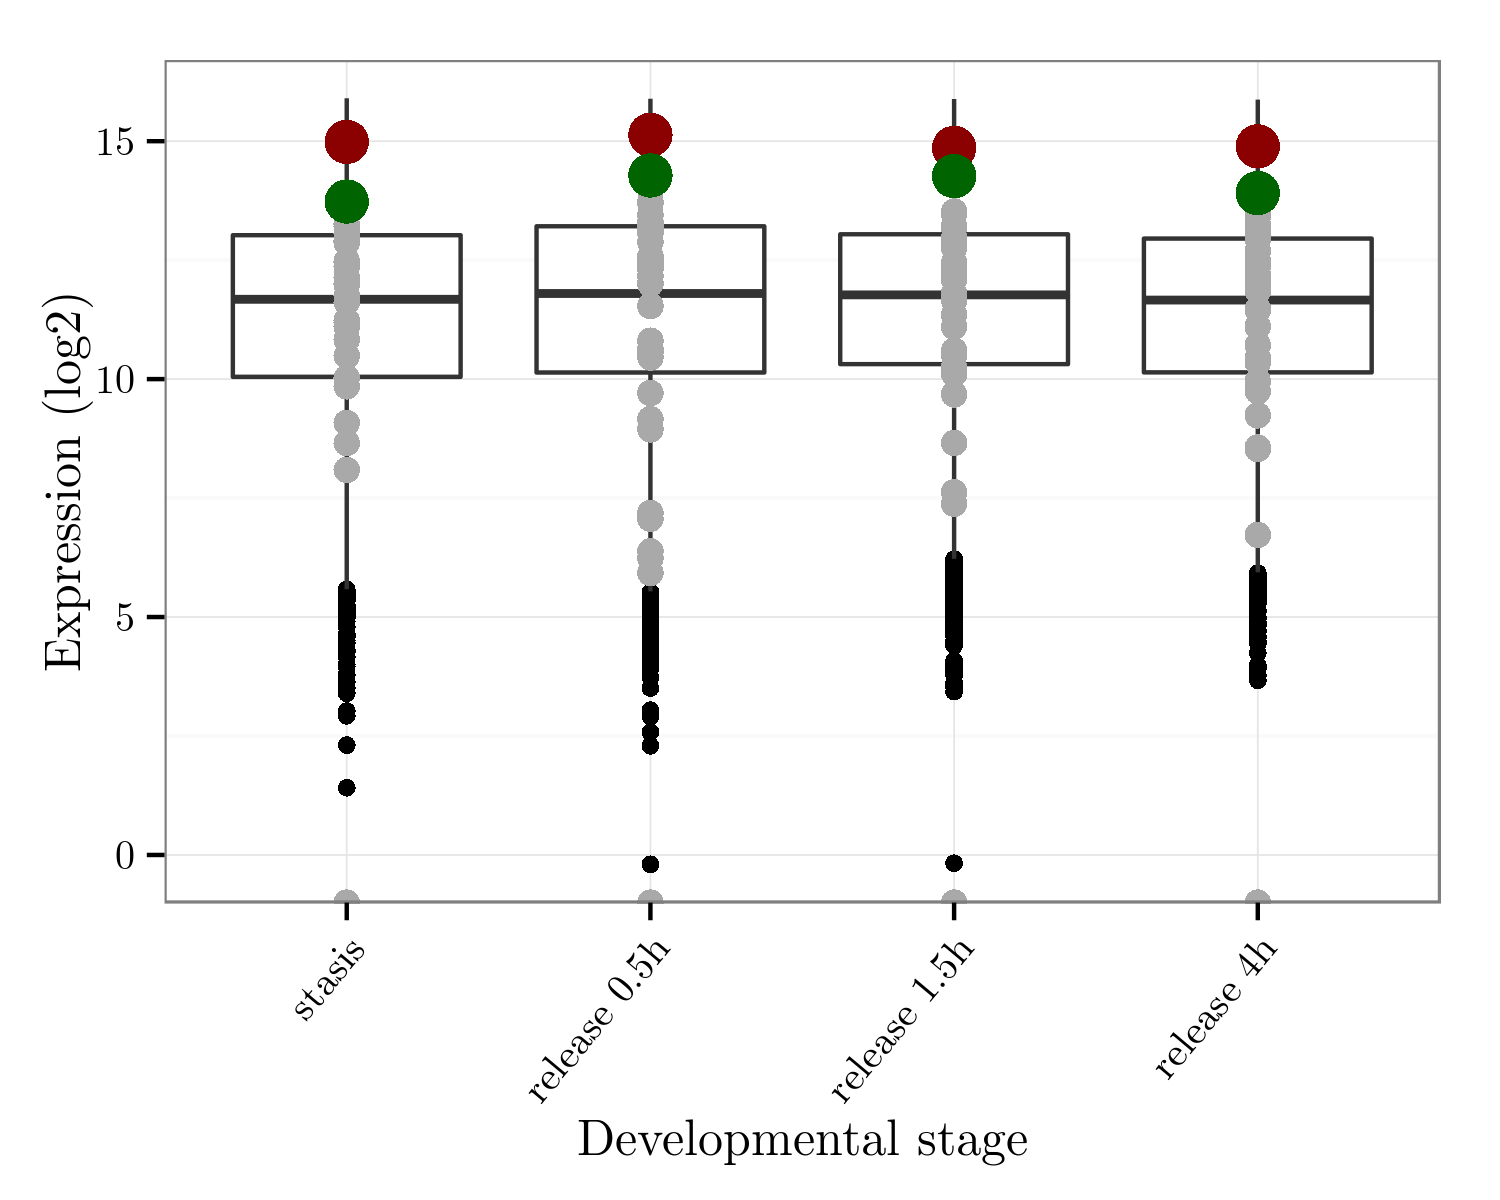
\includegraphics[width=1\linewidth]{pngs/stasisRelease_Dot1_expression_allgenes_SETs.png}
			\caption{Expression after release of growth arrest condition.}
		\end{subfigure}
		\caption{Expression values of Dot1 and Bre1 enzymes during (A) normal \textit{Oikopleura} development and growth arrest, and (B) after release from the growth arrest condition.
		Red: Bre1;
		Green: Dot1;
			{\footnotesize
			Expression values were transformed with a logarithm of base 2.
			}
		}
		\label{fig:Dot1_Bre1_GA_expression}
	\end{figure}
	
	
	
	
	
	Use of K79 methylation (K79me) during Oikopleura dioica's life cycle.
	Assessed by western blot on whole animals (Figure \ref{fig:k79me}a).
	Developmental stages with a predominant use of endocycles show increased levels of K79 methylation.
	Developmental stages with a predominant use of the canonical eukaryotic cell cycle mode show decreased levels of K79 methylation.
	
	(Figure \ref{fig:k79me}b).	
	H2BK123ub and H3K79 methylation – negative feedback regulation.
	Reduction of H3S10p – reduced cell proliferation.
	
	
	\begin{figure}
		\centering
		\begin{subfigure}{.5\textwidth}
			\centering
			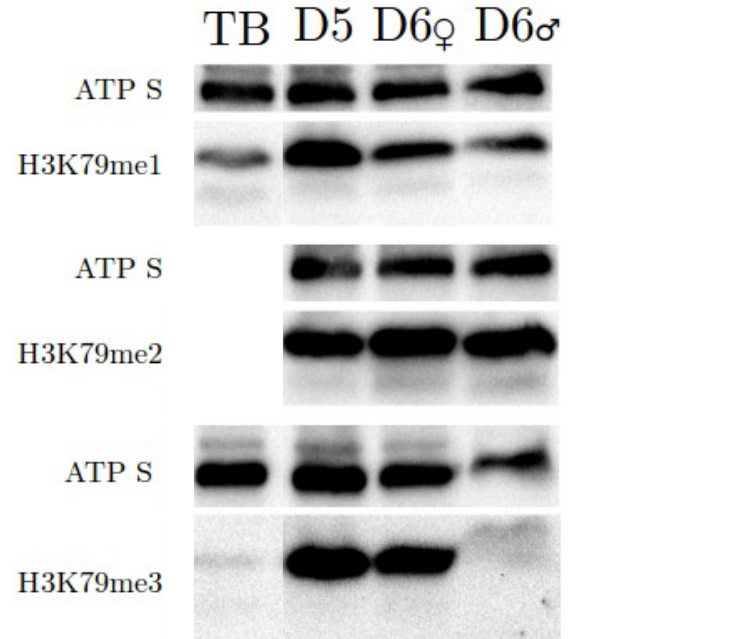
\includegraphics[width=1\linewidth]{pngs/K79me_WT.png}
			\caption{K79me in selected developmental stages.}
		\end{subfigure}%
		\begin{subfigure}{.5\textwidth}
			\centering
			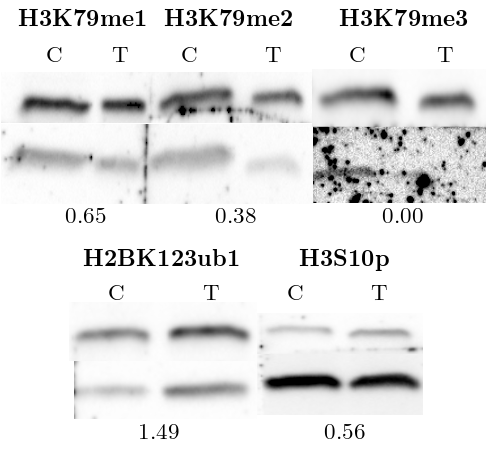
\includegraphics[width=1\linewidth]{pngs/TB_Dot1_in.png}
			\caption{Tailbud stage.}
		\end{subfigure}
		\begin{subfigure}{.5\textwidth}
			\centering
			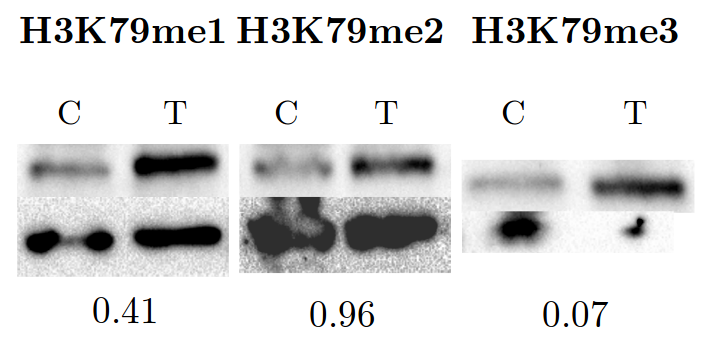
\includegraphics[width=1\linewidth]{pngs/D5_Dot1_in.png}
			\caption{D5 stage.}
		\end{subfigure}
		\caption{Quantification of K79 methylation states during selected developmental stages of \textit{Oikopleura dioica}'s life cycle and in Dot1in-treated animals by Western blot.
			{\footnotesize
				In (b) and (c), values under blots show the relative amounts compared with control normalized by ATP synthase $beta$ subunit (upper band). C - DMSO-treated control animals; T - Dot1in-treated animals.
			}
		}
		\label{fig:k79me}
	\end{figure}


Evidence for low H3K79me in \textit{Oikopleura}:
	RNA level:
		Dot1 expression is lower during endocyling stages
		Growth arrested animals have higher Dot1 expression than normal development
		Bre1 and Rad1 expression is low
	Protein level:
		MS data: H3K79me1 is very high, H3K79me2 lower and H3K79me3 not detected (in day 4 and 6 males)
		Western blots
		
H2BK123ub1 and H3K79me positive feedback


Experiments:
	Dot1 inhibition in early stages or growth arrested animals
	Dot1 overexpression in late stages
	
	Compare normal/dense expression pattern of all genes/methyltransferases/Dot1
	
	GO of H3K79me2/3 bound genes


\clearpage

%=========================================================================%
\chapter{Discussion}
%=========================================================================%



Higher states of K79 methylation accumulate with cell age \cite{DeVos2011}. What are the implications of this in an chordate with a extremely short cell cycle and fast cell division as \textit{Oikopleura}?


Dot1 is more expressed when cultured densely, which might indicate that 
Interestingly, the stage with least Dot1 expression is the testis, where the H3.t H3 variant is more expressed and the K79 residue is not present.

Bre1, the ubiquitin ligase of H2BK123 in yeast and mammals is present in \textit{Oikopleura}, but its expression is not ubiquitous unlike Dot1L. Bre1 is expressed in early stages, although not present maternally (detected earliest in tailbud animals) until day 3. It is not expressed in Day 4, but it is again in Day 5 and has its highest point of expression in the male testis. It is not expressed in the female gonad.

From MS data, H3K79me1/2 were detected, but not me3. me1 is much higher (is the most abundant of all histone PTMs) than me2 \cite{Moosmann2011}, possibly indicating that the state of H3K79me is one of "young cells", marked by low overall levels of H3K79me.

H2Bub was not quantified in MS.


\clearpage

%=========================================================================%
\chapter{Conclusions and Future Perspectives}
%=========================================================================%




replicates and ChIP-seq data -> more resolution -> more confidence 
Confirmation with ChIP-qPCR
Functional characterization of identified E2F binding sites 
\textit{in vivo} reporter constructs through transgenesis is not yet possible
alternatively,
injections in closely related (or not) species (e.g. Ciona intestinalis)
\textit{in vitro} assays of reporter with luciferase.




dsRNA knockout
overexpression

Possible role of Dot1 and K79 methylation in the regulation of biological processes known to involve deregulation of replication. Cancer




Regulation at both transcriptional and epigenetic levels is required and probably both play a role in the regulation and transition between \textit{Oikopleura}'s cell cycle modes.



\cleardoublepage
%=========================================================================%
%
% The bibliography
%
%=========================================================================%
\bibliographystyle{plain}
\bibliography{/data/Documents/Mendeley/library.bib}


\cleardoublepage
%=========================================================================%
% Appendix
%=========================================================================%
\begin{appendices}
	\chapter{Abbreviations}
		\begin{description}
			\item[aa] Amino acid
			\item[APC/C] Anaphase promoting complex
			\item[bp] Nucleotide base pair
			\item[CDK] Cyclin-dependent Kinase
			\item[CDS] Coding sequence of genes
			\item[ChIP] Chromatin immunoprecipitation
			\item[ChIP-ER] ChIP-enriched region
			\item[ChIP-seq] Chromatin immunoprecipitation followed by high-throughput sequencing
			\item[DNA] Deoxyribonucleic acid
			\item[kD] Kilo Dalton
			\item[$\mu$L, mL, L] Microlitre, Mililitre and Litre, respectively
			\item[O/N] Over night
			\item[R/T] Room temperature
			\item[RC] pre-Replication Complex
			\item[TF] Transcription factor
			\item[UTR] Untranslated regions of genes
			\item[V] Volt
		\end{description}

	\chapter{PCR primers}
		\label{appendixQPCRprimers}

	\chapter{Gene Ontology terms associated with genes putatively regulated by E2F factors}
	
	\chapter{List of key cell cycle regulators putatively regulated by E2F factors}	
	\label{list_key_cell_cycle_regulators}

\end{appendices}


\end{document}
